% Main content goes here
\chapter{Calculus I}
\section{Intermediate Value Theorem}

The Intermediate Value Theorem expresses a fundamental property of
continuous functions: a continuous graph cannot move from one height to
another without passing through every height in between.

\begin{theorem}[Intermediate Value Theorem]
    Let \(f\) be continuous on the closed interval \([a,b]\), and let \(N\)
    be any number between \(f(a)\) and \(f(b)\).  Then there exists at least
    one number \(c\in[a,b]\) such that
    \[
        f(c)=N.
    \]
    In particular, if \(N\) lies strictly between \(f(a)\) and \(f(b)\),
    then \(c\) may be chosen in \((a,b)\).
\end{theorem}
\begin{proof}
    If \(N=f(a)\) or \(N=f(b)\), choose \(c=a\) or \(c=b\), respectively.
    It therefore remains to consider the case in which \(N\) lies strictly
    between the endpoint values.  Without loss of generality, suppose that
    \[
        f(a)<N<f(b).
    \]
    (If \(f(b)<N<f(a)\), apply the following argument to \(-f\).)

    Define
    \[
        S=\{x\in[a,b]:f(x)\leq N\}.
    \]
    The set \(S\) is nonempty because \(a\in S\), and it is bounded above
    by \(b\).  By the completeness property of the real numbers, \(S\) has
    a least upper bound; let
    \[
        c=\sup S.
    \]
    Continuity at \(a\), together with \(f(a)<N\), shows that points just
    to the right of \(a\) belong to \(S\), so \(c>a\).  Similarly,
    continuity at \(b\), together with \(f(b)>N\), shows that no point
    sufficiently close to \(b\) from the left belongs to \(S\), so
    \(c<b\).  Thus \(c\in(a,b)\).

    We now prove that \(f(c)=N\).  Suppose first that \(f(c)<N\).  By
    continuity at \(c\), there is some \(\delta>0\) such that
    \(f(x)<N\) whenever \(|x-c|<\delta\).  Since \(c<b\), we may choose
    \(x\in(c,b]\) with \(|x-c|<\delta\).  Then \(x\in S\), contradicting
    the fact that \(c\) is an upper bound of \(S\).

    Suppose instead that \(f(c)>N\).  Continuity at \(c\) gives some
    \(\delta>0\) such that \(f(x)>N\) whenever \(|x-c|<\delta\).  Because
    \(c=\sup S\), there must be an \(x\in S\) satisfying
    \(c-\delta<x\leq c\); otherwise, \(c-\delta\) would be an upper bound
    of \(S\) smaller than \(c\).  But this \(x\) satisfies both
    \(f(x)\leq N\), since \(x\in S\), and \(f(x)>N\), by continuity.  This
    is a contradiction.

    Neither \(f(c)<N\) nor \(f(c)>N\) is possible.  Therefore \(f(c)=N\),
    as required.
\end{proof}

\section{Derivatives of Trigonometric Functions}
Two of the most essential formulas are 
\[
    \lim_{h \to 0} \frac{\sin h}{h} = 1 \quad \text{and} \quad \lim_{h \to 0} \frac{\cos h - 1}{h} = 0.   
\]
By this, and the definition of derivatives, we can obtain
\begin{table}[H]
    \centering
    \begin{tabular}{ll}
        \toprule
            \(\frac{\mathrm{d}}{\mathrm{d}x} \sin x = \cos x \)  & \(\frac{\mathrm{d}}{\mathrm{d}x} \csc x = - \csc x \cot x \)   \\
            \(\frac{\mathrm{d}}{\mathrm{d}x} \cos x = -\sin x \)  & \(\frac{\mathrm{d}}{\mathrm{d}x} \sec x = \sec x \tan x\)   \\
            \(\frac{\mathrm{d}}{\mathrm{d}x} \tan x = \sec ^2 x\)  & \(\frac{\mathrm{d}}{\mathrm{d}x} \cot x = - \csc ^2 x\)   \\
        \bottomrule
    \end{tabular}
    \caption{Derivatives of Trigonometric Functions}
    \label{tab:d of trig}
\end{table} 

\begin{theorem}[Two fundamental trigonometric limits]
    When angles are measured in radians,
    \[
        \lim_{h \to 0} \frac{\sin h}{h} = 1
        \qquad \text{and} \qquad
        \lim_{h \to 0} \frac{\cos h - 1}{h} = 0.
    \]
\end{theorem}
\begin{proof}
    We first prove the geometric inequality needed for the first limit.
    \begin{subproof}[Geometric inequality]
        Let \(0<h<\frac{\pi}{2}\).  In the following unit-circle diagram,
        \(OA=OB=1\), the line \(AC\) is tangent to the circle at \(A\), and
        \(\angle AOB=h\).
        \begin{center}
            \begin{tikzpicture}[
                line cap=round,
                line join=round,
                every node/.style={font=\small},
                region label/.style={
                    rounded corners=2pt,
                    inner sep=4pt,
                    font=\small
                }
            ]
                \def\angleh{38}
                \coordinate (O) at (0,0);
                \coordinate (A) at (3,0);
                \coordinate (B) at ({3*cos(\angleh)},{3*sin(\angleh)});
                \coordinate (C) at (3,{3*tan(\angleh)});
                \coordinate (D) at ({3*cos(\angleh)},0);

                % The three nested regions whose areas are compared.
                \fill[orange!25] (O)--(A)--(C)--cycle;
                \fill[TealBlue!22]
                    (O)--(A) arc[start angle=0,end angle=\angleh,radius=3]--cycle;
                \fill[SeaGreen!32] (O)--(A)--(B)--cycle;

                \draw[thick] (O)--(A)--(C)--cycle;
                \draw[thick,SeaGreen!65!black] (A)--(B);
                \draw[thick] (O)--(B);
                \draw[gray!55] (A) arc[start angle=0,end angle=90,radius=3];
                \draw[very thick,TealBlue!75!black]
                    (A) arc[start angle=0,end angle=\angleh,radius=3];
                \draw[dashed,gray!80] (B)--(D);
                \draw pic[
                    draw,
                    ->,
                    angle radius=9mm,
                    angle eccentricity=1.3,
                    "$h$"
                ] {angle=A--O--B};

                % Right-angle markers at the tangent point and the altitude.
                \draw ($(A)+(-0.18,0)$)--($(A)+(-0.18,0.18)$)--($(A)+(0,0.18)$);
                \draw ($(D)+(0.16,0)$)--($(D)+(0.16,0.16)$)--($(D)+(0,0.16)$);

                \node[below left] at (O) {\(O\)};
                \node[below right] at (A) {\(A\)};
                \node[above left] at (B) {\(B\)};
                \node[right] at (C) {\(C\)};
                \node[below] at (D) {\(D\)};
                \node[below] at ($(O)!0.37!(A)$) {\(1\)};
                \node[above left] at ($(O)!0.42!(B)$) {\(1\)};
                \node[right,inner sep=1pt] at ($(B)!0.52!(D)$)
                    {\(\sin h\)};
                \node[right] at ($(A)!0.5!(C)$) {\(\tan h\)};

                \node[
                    region label,
                    draw=SeaGreen!65!black,
                    fill=SeaGreen!12,
                    anchor=west
                ] at (0,-0.78) {\(\triangle OAB:\ \frac12\sin h\)};
                \node[
                    region label,
                    draw=TealBlue!70!black,
                    fill=TealBlue!10,
                    anchor=west
                ] at (2.65,-0.78) {sector \(OAB:\ \frac12h\)};
                \node[
                    region label,
                    draw=orange!70!black,
                    fill=orange!12,
                    anchor=west
                ] at (5.5,-0.78) {\(\triangle OAC:\ \frac12\tan h\)};
            \end{tikzpicture}
        \end{center}
        Indeed, \(OA=1\) and the altitude \(BD=\sin h\), so
        \[
            [OAB]=\frac12(OA)(BD)=\frac12\sin h.
        \]
        The sector has area \(h/2\) because its radius is \(1\), while
        \(AC=\tan h\) gives \([OAC]=\frac12\tan h\).  Since the three shaded
        regions are nested, their areas satisfy
        \[
            \underbrace{\frac{1}{2}\sin h}_{[OAB]}
            \leq \frac{1}{2}h
            \leq
            \underbrace{\frac{1}{2}\tan h}_{[OAC]}.
        \]
        Since \(\sin h>0\) and \(\cos h>0\), these inequalities imply
        \[
            \cos h \leq \frac{\sin h}{h} \leq 1.
        \]
    \end{subproof}

    The function \(\sin h/h\) is even, so for
    \(0<|h|<\frac{\pi}{2}\) the preceding inequality becomes
    \[
        \cos |h| \leq \frac{\sin h}{h} \leq 1.
    \]
    The same geometric comparison gives
    \(\lvert\sin x\rvert\leq\lvert x\rvert\) near \(0\).  Consequently,
    \[
        0\leq 1-\cos|h|
        =2\sin^2\!\left(\frac{|h|}{2}\right)
        \leq \frac{h^2}{2},
    \]
    so \(\cos|h|\to1\) as \(h\to0\).  The squeeze theorem therefore yields
    \[
        \lim_{h\to0}\frac{\sin h}{h}=1.
    \]

    For the second limit, the identity
    \(\cos h-1=-2\sin^2(h/2)\) gives
    \[
        \frac{\cos h-1}{h}
        =-\sin\!\left(\frac{h}{2}\right)
          \frac{\sin(h/2)}{h/2}.
    \]
    Moreover, \(\lvert\sin(h/2)\rvert\leq |h|/2\), and hence
    \(\sin(h/2)\to0\).  Together with the first limit, this proves
    \[
        \lim_{h\to0}\frac{\cos h-1}{h}
        =-(0)(1)=0.
    \]
\end{proof}

\section{Derivatives of Logarithmic and Inverse Trigonometric Functions}
\subsection{Logarithmic Functions}
\begin{theorem}
    \[
        \frac{\mathrm{d}}{\mathrm{d}x} \log _b x = \frac{1}{x \ln b}. 
    \]
\end{theorem}
\begin{proof}
    Let
    \[
        y=\log_b x,
    \]
    where \(x>0\), \(b>0\), and \(b\neq1\).  By the definition of a
    logarithm, this is equivalent to
    \[
        b^y=x.
    \]
    Differentiating both sides implicitly with respect to \(x\) gives
    \[
        b^y\ln b\,\frac{\mathrm{d}y}{\mathrm{d}x}=1.
    \]
    Since \(b^y=x\), it follows that
    \[
        \frac{\mathrm{d}y}{\mathrm{d}x}
        =\frac{1}{b^y\ln b}
        =\frac{1}{x\ln b}.
    \]
    Therefore,
    \[
        \frac{\mathrm{d}}{\mathrm{d}x}\log_b x
        =\frac{1}{x\ln b}.
    \]
    \begin{remark}
        \[
            \frac{\mathrm{d}}{\mathrm{d}x} b^x = b^x \ln x . 
        \]
    \end{remark}
\end{proof}

\begin{theorem}
    \[
        \frac{\mathrm{d}}{\mathrm{d}x} \ln \vert x \vert = \frac{1}{x}.  
    \]
\end{theorem}

\begin{definition}
    \(e = \lim_{x \to 0} (1 + x)^{\frac{1}{x}} = \lim_{n \to \infty} \left( 1 + \frac{1}{n} \right)^n   \). 
\end{definition}

\subsection{Trigonometric Functions}

\begin{table}[H]
    \centering
    \begin{tabular}{ll}
        \toprule
        \(\displaystyle \frac{\mathrm{d}}{\mathrm{d}x}\sin^{-1}x
            =\frac{1}{\sqrt{1-x^2}}\)
        & \(\displaystyle \frac{\mathrm{d}}{\mathrm{d}x}\cos^{-1}x
            =-\frac{1}{\sqrt{1-x^2}}\) \\
        \(\displaystyle \frac{\mathrm{d}}{\mathrm{d}x}\tan^{-1}x
            =\frac{1}{1+x^2}\)
        & \(\displaystyle \frac{\mathrm{d}}{\mathrm{d}x}\cot^{-1}x
            =-\frac{1}{1+x^2}\) \\
        \(\displaystyle \frac{\mathrm{d}}{\mathrm{d}x}\sec^{-1}x
            =\frac{1}{\lvert x\rvert\sqrt{x^2-1}}\)
        & \(\displaystyle \frac{\mathrm{d}}{\mathrm{d}x}\csc^{-1}x
            =-\frac{1}{\lvert x\rvert\sqrt{x^2-1}}\) \\
        \bottomrule
    \end{tabular}
    \caption{Derivatives of inverse trigonometric functions}
    \label{tab:derivatives-of-inverse-trig}
\end{table}

\begin{theorem}
    For \(-1<x<1\),
    \[
        \frac{\mathrm{d}}{\mathrm{d}x}\sin^{-1}x
        =\frac{1}{\sqrt{1-x^2}}.
    \]
\end{theorem}
\begin{proof}
    Let
    \[
        y=\sin^{-1}x.
    \]
    Since the range of \(\sin^{-1}\) is
    \(\left[-\frac{\pi}{2},\frac{\pi}{2}\right]\), this is equivalent to
    \[
        \sin y=x,
        \qquad
        -\frac{\pi}{2}\leq y\leq\frac{\pi}{2}.
    \]
    Differentiating \(\sin y=x\) implicitly with respect to \(x\) gives
    \[
        \cos y\,\frac{\mathrm{d}y}{\mathrm{d}x}=1,
    \]
    and hence
    \[
        \frac{\mathrm{d}y}{\mathrm{d}x}=\frac{1}{\cos y}.
    \]
    On the stated range of \(y\), we have \(\cos y\geq0\).  Therefore,
    using \(\sin y=x\) and the identity
    \(\sin^2y+\cos^2y=1\),
    \[
        \cos y
        =\sqrt{1-\sin^2y}
        =\sqrt{1-x^2}.
    \]
    Substitution yields
    \[
        \frac{\mathrm{d}}{\mathrm{d}x}\sin^{-1}x
        =\frac{\mathrm{d}y}{\mathrm{d}x}
        =\frac{1}{\sqrt{1-x^2}}.
    \]
\end{proof}

\section{Hyperbolic Functions}

\providecommand{\sech}{\operatorname{sech}}
\providecommand{\csch}{\operatorname{csch}}
\providecommand{\arsinh}{\operatorname{arsinh}}
\providecommand{\arcosh}{\operatorname{arcosh}}
\providecommand{\artanh}{\operatorname{artanh}}
\providecommand{\arcoth}{\operatorname{arcoth}}
\providecommand{\arsech}{\operatorname{arsech}}
\providecommand{\arcsch}{\operatorname{arcsch}}

Hyperbolic functions are combinations of the exponential functions
\(e^x\) and \(e^{-x}\).  They are analogous to trigonometric functions,
but they are associated with the hyperbola \(u^2-v^2=1\) rather than the
circle \(u^2+v^2=1\).

\begin{definition}
    For every real number \(x\), define
    \[
        \sinh x=\frac{e^x-e^{-x}}{2},
        \qquad
        \cosh x=\frac{e^x+e^{-x}}{2},
        \qquad
        \tanh x=\frac{\sinh x}{\cosh x}.
    \]
    The reciprocal hyperbolic functions are
    \[
        \sech x=\frac{1}{\cosh x},
        \qquad
        \csch x=\frac{1}{\sinh x},
        \qquad
        \coth x=\frac{\cosh x}{\sinh x}.
    \]
    Thus \(\csch x\) and \(\coth x\) are undefined at \(x=0\), whereas
    the other four functions are defined for every real \(x\).
\end{definition}

The following graphs show the characteristic shapes of all six functions.
The dashed lines are horizontal or vertical asymptotes.

\begin{figure}[H]
    \centering
    \begin{tikzpicture}
        \begin{groupplot}[
            group style={group size=2 by 3, horizontal sep=1.25cm,
                vertical sep=1.25cm},
            width=0.45\textwidth,
            height=0.29\textwidth,
            axis lines=middle,
            xmin=-3, xmax=3,
            samples=160,
            grid=both,
            minor tick num=1,
            xlabel={\(x\)},
            tick label style={font=\scriptsize},
            title style={font=\small}
        ]
        \nextgroupplot[title={\(y=\sinh x\)}, ymin=-5, ymax=5]
            \addplot[very thick,TealBlue,domain=-2.4:2.4]
                {(exp(x)-exp(-x))/2};
        \nextgroupplot[title={\(y=\cosh x\)}, ymin=-0.5, ymax=5]
            \addplot[very thick,orange!85!black,domain=-2.4:2.4]
                {(exp(x)+exp(-x))/2};
        \nextgroupplot[title={\(y=\tanh x\)}, ymin=-1.5, ymax=1.5]
            \addplot[dashed,gray,domain=-3:3] {1};
            \addplot[dashed,gray,domain=-3:3] {-1};
            \addplot[very thick,SeaGreen!75!black,domain=-3:3]
                {(exp(x)-exp(-x))/(exp(x)+exp(-x))};
        \nextgroupplot[title={\(y=\coth x\)}, ymin=-4, ymax=4]
            \addplot[dashed,gray,domain=-3:3] {1};
            \addplot[dashed,gray,domain=-3:3] {-1};
            \addplot[dashed,gray] coordinates {(0,-4) (0,4)};
            \addplot[very thick,violet,domain=-3:-0.27]
                {(exp(x)+exp(-x))/(exp(x)-exp(-x))};
            \addplot[very thick,violet,domain=0.27:3]
                {(exp(x)+exp(-x))/(exp(x)-exp(-x))};
        \nextgroupplot[title={\(y=\sech x\)}, ymin=-0.25, ymax=1.25]
            \addplot[dashed,gray,domain=-3:3] {0};
            \addplot[very thick,blue!70!black,domain=-3:3]
                {2/(exp(x)+exp(-x))};
        \nextgroupplot[title={\(y=\csch x\)}, ymin=-4, ymax=4]
            \addplot[dashed,gray,domain=-3:3] {0};
            \addplot[dashed,gray] coordinates {(0,-4) (0,4)};
            \addplot[very thick,red!75!black,domain=-3:-0.27]
                {2/(exp(x)-exp(-x))};
            \addplot[very thick,red!75!black,domain=0.27:3]
                {2/(exp(x)-exp(-x))};
        \end{groupplot}
    \end{tikzpicture}
    \caption{Graphs of the six hyperbolic functions}
    \label{fig:hyperbolic-functions}
\end{figure}

The functions \(\cosh x\) and \(\sech x\) are even; the other four are
odd.  Their ranges are summarized below.
\begin{table}[H]
    \centering
    \begin{tabular}{lll}
        \toprule
        Function & Domain & Range \\
        \midrule
        \(\sinh x\) & \(\mathbb{R}\) & \(\mathbb{R}\) \\
        \(\cosh x\) & \(\mathbb{R}\) & \([1,\infty)\) \\
        \(\tanh x\) & \(\mathbb{R}\) & \((-1,1)\) \\
        \(\coth x\) & \(\mathbb{R}\setminus\{0\}\)
            & \(( -\infty,-1)\cup(1,\infty)\) \\
        \(\sech x\) & \(\mathbb{R}\) & \((0,1]\) \\
        \(\csch x\) & \(\mathbb{R}\setminus\{0\}\)
            & \(\mathbb{R}\setminus\{0\}\) \\
        \bottomrule
    \end{tabular}
    \caption{Domains and ranges of hyperbolic functions}
    \label{tab:hyperbolic-domains-ranges}
\end{table}

\subsection{Hyperbolic Identities}

The exponential definitions give the fundamental identity
\[
    \cosh^2x-\sinh^2x=1.
\]
Dividing it by \(\cosh^2x\) or \(\sinh^2x\), respectively, gives
\[
    1-\tanh^2x=\sech^2x,
    \qquad
    \coth^2x-1=\csch^2x.
\]
The addition and subtraction formulas are
\begin{align*}
    \sinh(x\pm y)&=\sinh x\cosh y\pm\cosh x\sinh y,\\
    \cosh(x\pm y)&=\cosh x\cosh y\pm\sinh x\sinh y,\\
    \tanh(x\pm y)&=\frac{\tanh x\pm\tanh y}
        {1\pm\tanh x\tanh y},
\end{align*}
whenever the denominator in the last expression is nonzero.  In
particular,
\[
    \sinh(2x)=2\sinh x\cosh x,
    \qquad
    \cosh(2x)=\cosh^2x+\sinh^2x.
\]

\subsection{Derivatives of Hyperbolic Functions}

For example, differentiating the exponential definition gives
\[
    \frac{\mathrm{d}}{\mathrm{d}x}\sinh x
    =\frac{e^x+e^{-x}}{2}=\cosh x.
\]
The remaining formulas follow in the same way, together with the quotient
and reciprocal rules.
\begin{table}[H]
    \centering
    \begin{tabular}{ll}
        \toprule
        \(\displaystyle (\sinh x)'=\cosh x\)
            & \(\displaystyle (\cosh x)'=\sinh x\) \\
        \(\displaystyle (\tanh x)'=\sech^2x\)
            & \(\displaystyle (\coth x)'=-\csch^2x\) \\
        \(\displaystyle (\sech x)'=-\sech x\tanh x\)
            & \(\displaystyle (\csch x)'=-\csch x\coth x\) \\
        \bottomrule
    \end{tabular}
    \caption{Derivatives of hyperbolic functions}
    \label{tab:hyperbolic-derivatives}
\end{table}

\subsection{Inverse Hyperbolic Functions}

An inverse hyperbolic function reverses a one-to-one branch of a
hyperbolic function.  We use the notation \(\arsinh x,\arcosh x\), and so
on; this avoids confusing an inverse function with a reciprocal.  For
example,
\[
    y=\arsinh x
    \quad\Longleftrightarrow\quad
    x=\sinh y.
\]
The function \(\cosh x\) is restricted to \([0,\infty)\) before it is
inverted, while \(\coth x\) is inverted separately on its negative and
positive branches.  The real principal branches are listed below.

\begin{table}[H]
    \centering
    \small
    \begin{tabular}{lll}
        \toprule
        Function & Domain & Range \\
        \midrule
        \(\arsinh x\) & \(\mathbb{R}\) & \(\mathbb{R}\) \\
        \(\arcosh x\) & \([1,\infty)\) & \([0,\infty)\) \\
        \(\artanh x\) & \((-1,1)\) & \(\mathbb{R}\) \\
        \(\arcoth x\) & \(( -\infty,-1)\cup(1,\infty)\)
            & \(\mathbb{R}\setminus\{0\}\) \\
        \(\arsech x\) & \((0,1]\) & \([0,\infty)\) \\
        \(\arcsch x\) & \(\mathbb{R}\setminus\{0\}\)
            & \(\mathbb{R}\setminus\{0\}\) \\
        \bottomrule
    \end{tabular}
    \caption{Domains and ranges of inverse hyperbolic functions}
    \label{tab:inverse-hyperbolic-domains-ranges}
\end{table}

To solve for an inverse hyperbolic function, write the original function
in terms of exponentials and solve the resulting quadratic equation.  For
example, if \(y=\arsinh x\), then
\[
    x=\frac{e^y-e^{-y}}{2}.
\]
Multiplying by \(2e^y\) and setting \(u=e^y>0\) gives
\[
    u^2-2xu-1=0.
\]
Only the positive root is possible, so
\[
    e^y=x+\sqrt{x^2+1},
    \qquad
    \arsinh x=\ln\!\left(x+\sqrt{x^2+1}\right).
\]
The same method gives the logarithmic forms
\begin{align*}
    \arcosh x&=\ln\!\left(x+\sqrt{x^2-1}\right), &&x\geq1,\\
    \artanh x&=\frac12\ln\!\left(\frac{1+x}{1-x}\right), &&|x|<1,\\
    \arcoth x&=\frac12\ln\!\left(\frac{x+1}{x-1}\right), &&|x|>1,\\
    \arsech x&=\ln\!\left(\frac{1+\sqrt{1-x^2}}{x}\right), &&0<x\leq1,\\
    \arcsch x&=\arsinh\!\left(\frac1x\right)
        =\ln\!\left(\frac1x+\sqrt{1+\frac1{x^2}}\right), &&x\neq0.
\end{align*}

Inverse-function differentiation is often simpler than differentiating
the logarithmic formulas.  If \(y=\arsinh x\), then
\[
    x=\sinh y,
    \qquad
    1=\cosh y\,\frac{\mathrm{d}y}{\mathrm{d}x}.
\]
Since \(\cosh y=\sqrt{1+\sinh^2y}=\sqrt{1+x^2}\), we obtain
\[
    \frac{\mathrm{d}}{\mathrm{d}x}\arsinh x
    =\frac{1}{\sqrt{1+x^2}}.
\]
Applying the same idea to the other inverse functions gives
\begin{table}[H]
    \centering
    \small
    \begin{tabular}{ll}
        \toprule
        \(\displaystyle (\arsinh x)'=\frac{1}{\sqrt{1+x^2}}\)
            & \(\displaystyle (\arcosh x)'=\frac{1}{\sqrt{x^2-1}},\quad x>1\) \\
        \(\displaystyle (\artanh x)'=\frac{1}{1-x^2},\quad |x|<1\)
            & \(\displaystyle (\arcoth x)'=\frac{1}{1-x^2},\quad |x|>1\) \\
        \(\displaystyle (\arsech x)'=-\frac{1}{x\sqrt{1-x^2}},\quad 0<x<1\)
            & \(\displaystyle (\arcsch x)'=-\frac{1}{|x|\sqrt{1+x^2}},\quad x\neq0\) \\
        \bottomrule
    \end{tabular}
    \caption{Derivatives of inverse hyperbolic functions}
    \label{tab:inverse-hyperbolic-derivatives}
\end{table}

\section{Maximum and Minimum Values}
\begin{theorem}[The Extreme Value Theorem]
    If \(f\) is continuous on a closed interval \([a, b]\), then \(f\) attains an absolute maximum value \(f(c)\) and an absolute minimum value \(f(d)\) at some numbers \(c\) and \(d\) in \([a, b]\).        
\end{theorem}

\begin{theorem}[Fermat's Theorem]
    If \(f\) has a local maximum or minimum at \(c\), and if \(f^{\prime} (c)\) exists, then \(f^{\prime} (c) = 0\).    
\end{theorem}
\begin{proof}
    Suppose first that \(f\) has a local minimum at \(c\).  Then there is
    some \(\delta>0\) such that
    \[
        f(c+h)\geq f(c)
        \qquad\text{whenever}\qquad |h|<\delta.
    \]
    For \(0<h<\delta\), it follows that
    \[
        \frac{f(c+h)-f(c)}{h}\geq0,
    \]
    whereas for \(-\delta<h<0\), division by the negative number \(h\)
    reverses the inequality and gives
    \[
        \frac{f(c+h)-f(c)}{h}\leq0.
    \]
    Taking the right-hand limit preserves the first inequality, so
    \[
        f'_+(c)
        =\lim_{h\to0^+}\frac{f(c+h)-f(c)}{h}
        \geq0.
    \]
    Similarly, taking the left-hand limit in the second inequality gives
    \[
        f'_-(c)
        =\lim_{h\to0^-}\frac{f(c+h)-f(c)}{h}
        \leq0.
    \]
    Because \(f'(c)\) exists, the two one-sided derivatives exist and are
    equal to the derivative:
    \[
        f'_-(c)=f'(c)=f'_+(c).
    \]
    Thus the same number \(f'(c)\) is both nonpositive and nonnegative;
    therefore \(f'(c)=0\).

    If \(f\) has a local maximum at \(c\), then \(f(c+h)\leq f(c)\) for
    all sufficiently small \(|h|\).  Hence the inequalities are reversed:
    \[
        f'_+(c)
        =\lim_{h\to0^+}\frac{f(c+h)-f(c)}{h}
        \leq0,
        \qquad
        f'_-(c)
        =\lim_{h\to0^-}\frac{f(c+h)-f(c)}{h}
        \geq0.
    \]
    Once again, differentiability at \(c\) implies
    \(f'_-(c)=f'(c)=f'_+(c)\), so \(f'(c)=0\).
\end{proof}

\begin{eg}[A local extremum at which the derivative does not exist]
    Consider
    \[
        f(x)=|x|.
    \]
    Since \(f(x)\geq0=f(0)\) for every \(x\), the function has an absolute,
    and therefore local, minimum at \(x=0\).  However,
    \[
        \lim_{h\to0^+}\frac{f(0+h)-f(0)}{h}
        =\lim_{h\to0^+}\frac{|h|}{h}=1,
    \]
    while
    \[
        \lim_{h\to0^-}\frac{f(0+h)-f(0)}{h}
        =\lim_{h\to0^-}\frac{|h|}{h}=-1.
    \]
    Thus \(f'(0)\) does not exist.  This example shows why the assumption
    that \(f'(c)\) exists is necessary in Fermat's Theorem: a function may
    have a local maximum or minimum at a point where it is not
    differentiable.
\end{eg}

\begin{definition}
    A \vocab{critical number} of a function \(f\) is a number \(c\) in the domain of \(f\) s.t. either \(f^{\prime} (c) = 0\) or \(f^{\prime} (c)\) does not exist.  
\end{definition}

Thus, we can rephrase Fermat's theorem:

\begin{theorem}[Fermat's theorem (Rephrased)]
    If \(f\) has a local maximum or minimum at \(c\), then \(c\) is a critical number of \(f\).    
\end{theorem}

Combining the Extreme Value Theorem with Fermat's Theorem gives the
following procedure for finding absolute extrema on a closed interval.

\begin{algorithm}[H]
    \caption{The Closed Interval Method}
    \label{alg:closed-interval-method}
    \KwIn{A function \(f\) that is continuous on \([a,b]\).}
    \KwOut{The absolute maximum and minimum values of \(f\) on \([a,b]\).}

    Find every critical number \(c\) of \(f\) in the open interval
    \((a,b)\); that is, find all \(c\) for which \(f'(c)=0\) or \(f'(c)\)
    does not exist\;

    Evaluate \(f\) at each critical number and at the two endpoints:
    \[
        f(a),f(c_1),f(c_2),\ldots,f(b).
    \]

    Compare these values\;

    The largest value is the absolute maximum value of \(f\) on
    \([a,b]\), and the smallest value is the absolute minimum value\;
\end{algorithm}

\section{The Mean Value Theorem}

\begin{theorem}[Rolle's Theorem]
    Let \(f\) be a function that satisfies the following hypotheses:
    \begin{enumerate}
        \item \(f\) is continuous on the closed interval \([a, b]\). 
        \item \(f\) is differentiable on the open interval \((a, b)\). 
        \item \(f(a) = f(b)\),     
    \end{enumerate} 
    Then there is a number \(c\) in \((a, b)\) s.t. \(f^{\prime} (c) = 0\).   
\end{theorem}
\begin{proof}
    Since \(f\) is continuous on the closed interval \([a,b]\), the
    Extreme Value Theorem guarantees that \(f\) attains both an absolute
    maximum and an absolute minimum on \([a,b]\).

    If these two extreme values are equal, then \(f\) is constant on
    \([a,b]\).  Hence \(f'(c)=0\) for every \(c\in(a,b)\), and the result
    follows.

    Now suppose that the absolute maximum and minimum values are not equal.
    Because \(f(a)=f(b)\), at least one of these extreme values differs from
    the common endpoint value.  The point at which that extreme value is
    attained can therefore be neither \(a\) nor \(b\); thus it is attained
    at some \(c\in(a,b)\).  This point \(c\) is a local maximum or local
    minimum of \(f\).  Since \(f\) is differentiable at every point of
    \((a,b)\), Fermat's Theorem gives
    \[
        f'(c)=0.
    \]
    Therefore, in all cases, there exists some \(c\in(a,b)\) such that
    \(f'(c)=0\).
\end{proof}

\begin{theorem}[Mean Value Theorem]
    Let \(f\) be continuous on the closed interval \([a,b]\) and
    differentiable on the open interval \((a,b)\).  Then there exists a
    number \(c\in(a,b)\) such that
    \[
        f'(c)=\frac{f(b)-f(a)}{b-a}.
    \]
\end{theorem}
\begin{proof}
    Define the auxiliary function
    \[
        g(x)=f(x)-\frac{f(b)-f(a)}{b-a}(x-a).
    \]
    Since \(f\) is continuous on \([a,b]\) and differentiable on
    \((a,b)\), the function \(g\) has the same properties.  Moreover,
    \[
        g(a)=f(a)
    \]
    and
    \[
        g(b)
        =f(b)-\frac{f(b)-f(a)}{b-a}(b-a)
        =f(a).
    \]
    Thus \(g(a)=g(b)\).  By Rolle's Theorem, there exists some
    \(c\in(a,b)\) such that \(g'(c)=0\).  Since
    \[
        g'(x)=f'(x)-\frac{f(b)-f(a)}{b-a},
    \]
    we obtain
    \[
        0=g'(c)=f'(c)-\frac{f(b)-f(a)}{b-a}.
    \]
    Therefore,
    \[
        f'(c)=\frac{f(b)-f(a)}{b-a},
    \]
    as required.
\end{proof}

\begin{theorem}[Zero Derivative Theorem]
    If \(f'(x)=0\) for every \(x\in(a,b)\), then \(f\) is constant on
    \((a,b)\).
\end{theorem}
\begin{proof}
    Let \(x_1,x_2\in(a,b)\) with \(x_1<x_2\).  Since \(f\) is
    differentiable on \((a,b)\), it is continuous on \([x_1,x_2]\) and
    differentiable on \((x_1,x_2)\).  By the Mean Value Theorem, there
    exists some \(c\in(x_1,x_2)\) such that
    \[
        \frac{f(x_2)-f(x_1)}{x_2-x_1}=f'(c)=0.
    \]
    Hence \(f(x_2)=f(x_1)\).  Because \(x_1\) and \(x_2\) were arbitrary,
    \(f\) is constant on \((a,b)\).
\end{proof}

\begin{corollary}
    Let \(f\) and \(g\) be differentiable on \((a,b)\).  If
    \[
        f'(x)=g'(x)
    \]
    for every \(x\in(a,b)\), then \(f\) and \(g\) differ by a constant;
    that is, there exists a constant \(C\) such that
    \[
        f(x)=g(x)+C
    \]
    for every \(x\in(a,b)\).
\end{corollary}
\begin{proof}
    Define \(h=f-g\).  Then \(h\) is differentiable on \((a,b)\), and
    for every \(x\in(a,b)\),
    \[
        h'(x)=f'(x)-g'(x)=0.
    \]
    By the Zero Derivative Theorem, \(h\) is constant on \((a,b)\).
    Therefore, there exists a constant \(C\) such that
    \[
        f(x)-g(x)=C,
    \]
    or equivalently \(f(x)=g(x)+C\), for every \(x\in(a,b)\).
\end{proof}

\section{What Derivatives Tell Us about the Shape of a Graph}

Derivatives provide information about the shape of a graph.  The sign of
the first derivative describes where a function rises or falls, while the
sign of the second derivative describes how the slope itself changes.

\subsection{Increasing and Decreasing Functions}

\begin{definition}
    Let \(f\) be defined on an interval \(I\).
    \begin{enumerate}
        \item The function \(f\) is \vocab{increasing} on \(I\) if
        \(f(x_1)<f(x_2)\) whenever \(x_1<x_2\) in \(I\).
        \item The function \(f\) is \vocab{decreasing} on \(I\) if
        \(f(x_1)>f(x_2)\) whenever \(x_1<x_2\) in \(I\).
    \end{enumerate}
\end{definition}

Recall that a \vocab{critical number} of \(f\) is a number \(c\) in the
domain of \(f\) for which \(f'(c)=0\) or \(f'(c)\) does not exist.  Critical
numbers divide the domain into intervals on which the sign of \(f'\) can be
examined.

\begin{theorem}[Increasing/Decreasing Test]
    Suppose that \(f\) is continuous on an interval \(I\) and differentiable
    at every interior point of \(I\).
    \begin{enumerate}
        \item If \(f'(x)>0\) throughout the interior of \(I\), then \(f\) is
        increasing on \(I\).
        \item If \(f'(x)<0\) throughout the interior of \(I\), then \(f\) is
        decreasing on \(I\).
    \end{enumerate}
\end{theorem}
\begin{proof}
    Let \(x_1<x_2\) be points in \(I\).  By the Mean Value Theorem, there is
    some \(c\in(x_1,x_2)\) such that
    \[
        f(x_2)-f(x_1)=f'(c)(x_2-x_1).
    \]
    Since \(x_2-x_1>0\), the difference \(f(x_2)-f(x_1)\) has the same sign
    as \(f'(c)\).  The two conclusions follow.
\end{proof}

\begin{theorem}[First Derivative Test]
    Suppose that \(c\) is a critical number of a function \(f\), and that
    \(f\) is continuous at \(c\) and differentiable on intervals immediately
    to the left and right of \(c\).
    \begin{enumerate}
        \item If \(f'\) changes from positive to negative at \(c\), then
        \(f\) has a local maximum at \(c\).
        \item If \(f'\) changes from negative to positive at \(c\), then
        \(f\) has a local minimum at \(c\).
        \item If \(f'\) has the same sign on both sides of \(c\), then
        \(f\) has no local extremum at \(c\).
    \end{enumerate}
\end{theorem}

Thus the First Derivative Test may be applied by finding the critical
numbers, placing them on a number line, determining the sign of \(f'\) on
each resulting interval, and recording every change of sign.

\subsection{Concavity and the Second Derivative}

\begin{definition}
    Let \(f\) be differentiable on an interval \(I\).
    \begin{enumerate}
        \item The graph of \(f\) is \vocab{concave upward} on \(I\) if
        \(f'\) is increasing on \(I\).
        \item The graph of \(f\) is \vocab{concave downward} on \(I\) if
        \(f'\) is decreasing on \(I\).
    \end{enumerate}
\end{definition}

Geometrically, a graph that is concave upward has increasing tangent
slopes, while a graph that is concave downward has decreasing tangent
slopes.  Consequently, if
\(f''(x)>0\) on an interval, then \(f\) is concave upward there; if
\(f''(x)<0\), then \(f\) is concave downward there.

\begin{definition}
    A point \((c,f(c))\) on the graph of a continuous function \(f\) is an
    \vocab{inflection point} if the graph changes concavity at \(c\).
\end{definition}

The equation \(f''(c)=0\), or the failure of \(f''(c)\) to exist, only
identifies a possible inflection point.  A change of concavity must still be
verified on the two sides of \(c\).

\begin{theorem}[Second Derivative Test]
    Suppose that \(f'(c)=0\) and that \(f''\) exists on an open interval
    containing \(c\).
    \begin{enumerate}
        \item If \(f''(c)>0\), then \(f\) has a local minimum at \(c\).
        \item If \(f''(c)<0\), then \(f\) has a local maximum at \(c\).
        \item If \(f''(c)=0\), the test is inconclusive: \(f\) may have a
        local maximum, a local minimum, or neither at \(c\).
    \end{enumerate}
\end{theorem}
\begin{proof}
    Suppose first that \(f''(c)>0\).  Since \(f'(c)=0\), the definition of
    the second derivative gives
    \[
        f''(c)=\lim_{x\to c}\frac{f'(x)-f'(c)}{x-c}
        =\lim_{x\to c}\frac{f'(x)}{x-c}>0.
    \]
    Hence, sufficiently close to \(c\), the quotient is positive.  It
    follows that \(f'(x)<0\) to the left of \(c\) and \(f'(x)>0\) to the
    right.  The First Derivative Test therefore gives a local minimum at
    \(c\).  If \(f''(c)<0\), the signs are reversed, so \(f\) has a local
    maximum at \(c\).

    When \(f''(c)=0\), no conclusion follows from this argument.  For
    example, at \(c=0\), the functions \(x^4\), \(-x^4\), and \(x^3\) have,
    respectively, a local minimum, a local maximum, and no local extremum,
    although the first and second derivatives at \(0\) are zero in every
    case.
\end{proof}

\section{L'H\^{o}pital's Rule}

L'H\^{o}pital's Rule is a method for evaluating limits whose direct
substitution produces one of the indeterminate forms
\[
    \frac{0}{0}
    \qquad\text{or}\qquad
    \frac{\infty}{\infty}.
\]
The word \emph{indeterminate} is important: these forms do not determine the
value of a limit by themselves.  The rule replaces the original quotient by
the quotient of the derivatives of its numerator and denominator.

\begin{theorem}[L'H\^{o}pital's Rule]
    Let \(f\) and \(g\) be differentiable on an open interval containing
    \(a\), except possibly at \(a\), and suppose that \(g'(x)\neq0\) near
    \(a\).  Assume either
    \[
        \lim_{x\to a}f(x)=\lim_{x\to a}g(x)=0
    \]
    or that \(\lvert f(x)\rvert\to\infty\) and
    \(\lvert g(x)\rvert\to\infty\) as \(x\to a\).  If
    \[
        \lim_{x\to a}\frac{f'(x)}{g'(x)}=L,
    \]
    where \(L\) may be finite or infinite, then
    \[
        \lim_{x\to a}\frac{f(x)}{g(x)}=L.
    \]
    The same conclusion holds for one-sided limits and for limits as
    \(x\to\pm\infty\), provided the corresponding hypotheses are satisfied.
\end{theorem}

For the \(0/0\) case, the main idea follows from the Cauchy Mean Value
Theorem.  If the functions are defined at \(a\) by \(f(a)=g(a)=0\), then for
each nearby \(x\) there is a point \(c\) between \(a\) and \(x\) such that
\[
    \frac{f(x)}{g(x)}
    =\frac{f(x)-f(a)}{g(x)-g(a)}
    =\frac{f'(c)}{g'(c)}.
\]
As \(x\to a\), the point \(c\to a\), which explains why the limit of the
derivative quotient determines the original limit.

\subsection{How to Apply the Rule}

\begin{enumerate}
    \item Substitute or otherwise verify that the quotient has the form
    \(0/0\) or \(\infty/\infty\).
    \item Differentiate the numerator and denominator separately.  Do not
    use the quotient rule.
    \item Evaluate the new limit.  If it is again indeterminate, the rule
    may be applied repeatedly, provided its hypotheses continue to hold.
\end{enumerate}

For example,
\[
    \lim_{x\to0}\frac{e^x-1}{x}
    =\lim_{x\to0}\frac{e^x}{1}=1,
\]
because the original quotient has the form \(0/0\).  Similarly,
\[
    \lim_{x\to\infty}\frac{x^2}{e^x}
    =\lim_{x\to\infty}\frac{2x}{e^x}
    =\lim_{x\to\infty}\frac{2}{e^x}=0.
\]

Other indeterminate forms must first be rewritten.  Products of the form
\(0\cdot\infty\) can often be expressed as quotients, while differences of
the form \(\infty-\infty\) may require a common denominator or
rationalization.  For powers of the forms \(0^0\), \(1^\infty\), or
\(\infty^0\), one usually takes logarithms before applying the rule.  For
instance, if
\[
    y=(1+x)^{1/x},
\]
then
\[
    \ln y=\frac{\ln(1+x)}{x},
    \qquad
    \lim_{x\to0}\ln y
    =\lim_{x\to0}\frac{1/(1+x)}{1}=1.
\]
Therefore,
\[
    \lim_{x\to0}(1+x)^{1/x}=e.
\]

\begin{remark}
    L'H\^{o}pital's Rule applies only after an indeterminate form has been
    verified.  It cannot be used directly for a quotient approaching, for
    example, \(0/5\) or \(3/0\).  It is also unnecessary when algebraic
    simplification, a standard limit, or the squeeze theorem gives a more
    direct solution.
\end{remark}

\chapter{Calculus II}

\section{The Fundamental Theorem of Calculus}

The Fundamental Theorem of Calculus connects the two central operations of
calculus: differentiation and integration.  Differentiation measures an
instantaneous rate of change, while a definite integral accumulates a
quantity over an interval.  The theorem shows that these operations are, in
an important sense, inverses of one another.

\subsection{Accumulation Functions}

Let \(f\) be continuous on \([a,b]\), and define
\[
    A(x)=\int_a^x f(t)\,\mathrm{d}t.
\]
The value \(A(x)\) is the signed area accumulated under the graph of \(f\)
from \(a\) to \(x\).  If \(x\) increases by a small amount \(h\), then
\[
    A(x+h)-A(x)=\int_x^{x+h}f(t)\,\mathrm{d}t.
\]
For small \(h\), this additional area is approximately \(f(x)h\), suggesting
that \(A'(x)=f(x)\).

\begin{theorem}[Fundamental Theorem of Calculus, Part I]
    If \(f\) is continuous on \([a,b]\) and
    \[
        A(x)=\int_a^x f(t)\,\mathrm{d}t,
    \]
    then \(A\) is continuous on \([a,b]\), differentiable on \((a,b)\), and
    \[
        A'(x)=f(x).
    \]
\end{theorem}
\begin{proof}
    Fix \(x\in(a,b)\).  For every sufficiently small nonzero \(h\),
    \[
        \frac{A(x+h)-A(x)}{h}
        =\frac{1}{h}\int_x^{x+h}f(t)\,\mathrm{d}t.
    \]
    By the Mean Value Theorem for Integrals, there is a point \(c_h\) between
    \(x\) and \(x+h\) such that
    \[
        \int_x^{x+h}f(t)\,\mathrm{d}t=f(c_h)h.
    \]
    Hence
    \[
        \frac{A(x+h)-A(x)}{h}=f(c_h).
    \]
    As \(h\to0\), we have \(c_h\to x\).  Continuity of \(f\) therefore
    gives
    \[
        A'(x)=\lim_{h\to0}f(c_h)=f(x).
    \]
    The continuity of \(A\) follows from the same local estimate for the
    integral over the short interval between \(x\) and \(x+h\).
\end{proof}

More generally, the chain rule gives the useful formula
\[
    \frac{\mathrm{d}}{\mathrm{d}x}
    \int_a^{g(x)}f(t)\,\mathrm{d}t
    =f\bigl(g(x)\bigr)g'(x).
\]
For example,
\[
    \frac{\mathrm{d}}{\mathrm{d}x}
    \int_1^{x^2}\sqrt{1+t^3}\,\mathrm{d}t
    =2x\sqrt{1+x^6}.
\]

\subsection{Evaluating Definite Integrals}

An \vocab{antiderivative} of \(f\) on an interval is a function \(F\) such
that \(F'(x)=f(x)\) throughout that interval.  Part II of the theorem turns
the evaluation of a definite integral into the problem of finding an
antiderivative.

\begin{theorem}[Fundamental Theorem of Calculus, Part II]
    If \(f\) is continuous on \([a,b]\) and \(F\) is any antiderivative of
    \(f\) on \([a,b]\), then
    \[
        \int_a^b f(x)\,\mathrm{d}x=F(b)-F(a).
    \]
\end{theorem}
\begin{proof}
    Define
    \[
        A(x)=\int_a^x f(t)\,\mathrm{d}t.
    \]
    By Part I, \(A'(x)=f(x)\).  Since \(F'(x)=f(x)\) as well, the function
    \(F-A\) has derivative zero and is therefore constant.  At \(x=a\),
    \(A(a)=0\), so
    \[
        F(x)-A(x)=F(a).
    \]
    Taking \(x=b\) and rearranging gives
    \[
        \int_a^b f(t)\,\mathrm{d}t=A(b)=F(b)-F(a).
    \]
\end{proof}

The notation
\[
    \left.F(x)\right|_a^b
    \qquad\text{or}\qquad
    \bigl[F(x)\bigr]_a^b
\]
means \(F(b)-F(a)\).  Thus, for example,
\[
    \int_0^2 (3x^2-4x+1)\,\mathrm{d}x
    =\left[x^3-2x^2+x\right]_0^2
    =2.
\]

\begin{remark}
    The definite integral represents signed accumulation: regions above the
    horizontal axis contribute positively, while regions below it contribute
    negatively.  Therefore, \(\int_a^b f(x)\,\mathrm{d}x\) need not equal
    the total geometric area between the graph and the axis.  To find total
    area, split the interval at the zeros of \(f\) and integrate
    \(\lvert f(x)\rvert\).
\end{remark}

\section{Strategy for Integration}

Integrals containing powers of trigonometric functions are usually handled
by saving one factor for the differential and rewriting the remaining
factors with a Pythagorean identity.  The appropriate choice depends mainly
on whether the exponents are odd or even.  In the following discussion,
\(m\) and \(n\) are nonnegative integers.

\subsection{Integrals of \(\sin^m x\cos^n x\)}

Consider
\[
    \int \sin^m x\cos^n x\,\mathrm{d}x.
\]
The identities used most often are
\[
    \sin^2x=1-\cos^2x,
    \qquad
    \cos^2x=1-\sin^2x,
\]
and the power-reduction formulas
\[
    \sin^2x=\frac{1-\cos(2x)}{2},
    \qquad
    \cos^2x=\frac{1+\cos(2x)}{2}.
\]

\begin{enumerate}
    \item If \(m\) is odd, save one factor of \(\sin x\), convert the
    remaining even power of sine into powers of cosine, and use
    \(u=\cos x\):
    \[
        \sin^m x
        =\bigl(1-\cos^2x\bigr)^{(m-1)/2}\sin x.
    \]

    \item If \(n\) is odd, save one factor of \(\cos x\), convert the
    remaining even power of cosine into powers of sine, and use
    \(u=\sin x\):
    \[
        \cos^n x
        =\bigl(1-\sin^2x\bigr)^{(n-1)/2}\cos x.
    \]

    \item If both \(m\) and \(n\) are even, repeatedly use the
    power-reduction formulas.  Product-to-sum identities may also simplify
    the resulting products of multiple-angle functions.
\end{enumerate}

If both exponents are odd, either of the first two substitutions works.  For
example,
\begin{align*}
    \int\sin^3x\cos^2x\,\mathrm{d}x
    &=\int\bigl(1-\cos^2x\bigr)\cos^2x\sin x\,\mathrm{d}x \\
    &=-\int(u^2-u^4)\,\mathrm{d}u
        \qquad (u=\cos x)\\
    &=-\frac{\cos^3x}{3}+\frac{\cos^5x}{5}+C.
\end{align*}

When both exponents are even, for instance,
\begin{align*}
    \int\sin^2x\cos^2x\,\mathrm{d}x
    &=\frac14\int\sin^2(2x)\,\mathrm{d}x \\
    &=\frac18\int\bigl(1-\cos(4x)\bigr)\,\mathrm{d}x \\
    &=\frac{x}{8}-\frac{\sin(4x)}{32}+C.
\end{align*}

\subsection{Integrals of \(\tan^m x\sec^n x\)}

Now consider
\[
    \int\tan^m x\sec^n x\,\mathrm{d}x.
\]
Here the useful identities and differentials are
\[
    \tan^2x=\sec^2x-1,
    \qquad
    \sec^2x=1+\tan^2x,
\]
\[
    \mathrm{d}(\tan x)=\sec^2x\,\mathrm{d}x,
    \qquad
    \mathrm{d}(\sec x)=\sec x\tan x\,\mathrm{d}x.
\]

\begin{enumerate}
    \item If \(n\) is even and \(n\geq2\), save one factor of
    \(\sec^2x\), convert the remaining even powers of secant into tangent,
    and use \(u=\tan x\).

    \item If \(m\) is odd and \(n\geq1\), save one factor of
    \(\sec x\tan x\), convert the remaining even power of tangent into
    secant, and use \(u=\sec x\).  This method is especially natural when
    \(n\) is odd.

    \item If neither pattern applies, rewrite the integrand using
    \(\tan^2x=\sec^2x-1\).  The result may reduce to powers of secant, for
    which power-reduction formulas or integration by parts can be used.  In
    the special case \(n=0\), rewriting tangent in terms of sine and cosine
    is often convenient.
\end{enumerate}

For example, because the power of secant is even,
\begin{align*}
    \int\tan^3x\sec^4x\,\mathrm{d}x
    &=\int\tan^3x\bigl(1+\tan^2x\bigr)\sec^2x\,\mathrm{d}x \\
    &=\int u^3(1+u^2)\,\mathrm{d}u
        \qquad (u=\tan x)\\
    &=\frac{\tan^4x}{4}+\frac{\tan^6x}{6}+C.
\end{align*}
On the other hand, when an odd power of tangent is paired with a secant
factor,
\begin{align*}
    \int\tan^3x\sec^3x\,\mathrm{d}x
    &=\int\bigl(\sec^2x-1\bigr)\sec^2x
        (\sec x\tan x)\,\mathrm{d}x \\
    &=\int(u^4-u^2)\,\mathrm{d}u
        \qquad (u=\sec x)\\
    &=\frac{\sec^5x}{5}-\frac{\sec^3x}{3}+C.
\end{align*}

The central principle in both families is to preserve a factor that matches
the differential of the chosen substitution, then use an identity to express
every remaining factor in terms of the new variable.

\subsection{Integrals of \(\tan x\) and \(\sec x\)}

The antiderivative of tangent follows immediately after writing tangent as a
quotient:
\begin{align*}
    \int\tan x\,\mathrm{d}x
    &=\int\frac{\sin x}{\cos x}\,\mathrm{d}x.
\end{align*}
Let \(u=\cos x\), so that \(\mathrm{d}u=-\sin x\,\mathrm{d}x\).  Then
\begin{align*}
    \int\tan x\,\mathrm{d}x
    &=-\int\frac{1}{u}\,\mathrm{d}u \\
    &=-\ln|u|+C \\
    &=-\ln|\cos x|+C
      =\ln|\sec x|+C.
\end{align*}

The integral of secant requires a useful algebraic trick.  Multiply the
integrand by \((\sec x+\tan x)/(\sec x+\tan x)\):
\begin{align*}
    \int\sec x\,\mathrm{d}x
    &=\int\sec x
      \frac{\sec x+\tan x}{\sec x+\tan x}\,\mathrm{d}x \\
    &=\int\frac{\sec^2x+\sec x\tan x}
                    {\sec x+\tan x}\,\mathrm{d}x.
\end{align*}
With \(u=\sec x+\tan x\), we have
\[
    \mathrm{d}u
    =\bigl(\sec x\tan x+\sec^2x\bigr)\,\mathrm{d}x.
\]
Therefore,
\begin{align*}
    \int\sec x\,\mathrm{d}x
    &=\int\frac{1}{u}\,\mathrm{d}u \\
    &=\ln|u|+C \\
    &=\ln|\sec x+\tan x|+C.
\end{align*}
These two formulas are worth remembering:
\[
    \boxed{\int\tan x\,\mathrm{d}x=\ln|\sec x|+C},
    \qquad
    \boxed{\int\sec x\,\mathrm{d}x
        =\ln|\sec x+\tan x|+C}.
\]

\subsection{Product-to-Sum Identities}

Products of trigonometric functions with different angles can often be
integrated more easily after they are converted into sums.  The principal
product-to-sum identities are
\begin{align*}
    \sin A\sin B
        &=\frac12\bigl[\cos(A-B)-\cos(A+B)\bigr],\\
    \cos A\cos B
        &=\frac12\bigl[\cos(A-B)+\cos(A+B)\bigr],\\
    \sin A\cos B
        &=\frac12\bigl[\sin(A+B)+\sin(A-B)\bigr],\\
    \cos A\sin B
        &=\frac12\bigl[\sin(A+B)-\sin(A-B)\bigr].
\end{align*}
They follow by adding or subtracting the angle-sum and angle-difference
formulas.  For example,
\[
    \cos(A-B)-\cos(A+B)=2\sin A\sin B.
\]

As an application,
\begin{align*}
    \int\sin(3x)\cos(2x)\,\mathrm{d}x
    &=\frac12\int\bigl[\sin(5x)+\sin x\bigr],\mathrm{d}x \\
    &=-\frac{\cos(5x)}{10}-\frac{\cos x}{2}+C.
\end{align*}
Thus, a product-to-sum identity is useful when an integrand contains a
product of the form
\[
    \sin(ax)\sin(bx),
    \qquad
    \cos(ax)\cos(bx),
    \qquad\text{or}\qquad
    \sin(ax)\cos(bx).
\]
The identity separates the product into terms that can be integrated
individually.

\subsection{Trigonometric Substitution}

Trigonometric substitution is useful for integrals involving square roots of
quadratic expressions.  The substitution is chosen so that a Pythagorean
identity removes the radical.  For \(a>0\), the three standard patterns are
\begin{center}
    \begin{tabular}{lll}
        \toprule
        Expression & Substitution & Identity used \\
        \midrule
        \(\sqrt{a^2-x^2}\)
            & \(x=a\sin\theta\)
            & \(1-\sin^2\theta=\cos^2\theta\) \\
        \(\sqrt{a^2+x^2}\)
            & \(x=a\tan\theta\)
            & \(1+\tan^2\theta=\sec^2\theta\) \\
        \(\sqrt{x^2-a^2}\)
            & \(x=a\sec\theta\)
            & \(\sec^2\theta-1=\tan^2\theta\) \\
        \bottomrule
    \end{tabular}
\end{center}

For example, if \(x=a\sin\theta\), then
\[
    \mathrm{d}x=a\cos\theta\,\mathrm{d}\theta
    \qquad\text{and}\qquad
    \sqrt{a^2-x^2}
    =a\sqrt{1-\sin^2\theta}
    =a\cos\theta,
\]
where \(-\pi/2\leq\theta\leq\pi/2\) is chosen so that
\(\cos\theta\geq0\).  Similarly, suitable choices of \(\theta\) give
\[
    \sqrt{a^2+x^2}=a\sec\theta
    \quad\text{when }x=a\tan\theta,
\]
and
\[
    \sqrt{x^2-a^2}=a\tan\theta
    \quad\text{when }x=a\sec\theta.
\]
Choosing an interval on which the relevant trigonometric functions have the
correct signs avoids introducing unnecessary absolute values.

The usual procedure is:
\begin{enumerate}
    \item Identify which of the three quadratic expressions occurs.
    \item Make the corresponding substitution and replace
    \(\mathrm{d}x\).
    \item Use a Pythagorean identity to eliminate the square root.
    \item Evaluate the resulting trigonometric integral.
    \item Rewrite the answer in terms of \(x\).
\end{enumerate}

For instance, consider
\[
    \int\sqrt{9-x^2}\,\mathrm{d}x.
\]
Set \(x=3\sin\theta\), with
\(-\pi/2\leq\theta\leq\pi/2\).  Then
\[
    \mathrm{d}x=3\cos\theta\,\mathrm{d}\theta,
    \qquad
    \sqrt{9-x^2}=3\cos\theta.
\]
Therefore,
\begin{align*}
    \int\sqrt{9-x^2}\,\mathrm{d}x
    &=9\int\cos^2\theta\,\mathrm{d}\theta \\
    &=\frac92\int(1+\cos2\theta)\,\mathrm{d}\theta \\
    &=\frac92\theta+\frac94\sin2\theta+C.
\end{align*}
Since \(\sin\theta=x/3\), we have
\[
    \theta=\sin^{-1}\!\left(\frac{x}{3}\right),
    \qquad
    \cos\theta=\frac{\sqrt{9-x^2}}{3}.
\]
Thus
\[
    \sin2\theta
    =2\sin\theta\cos\theta
    =\frac{2x\sqrt{9-x^2}}{9},
\]
and the final result is
\[
    \boxed{
        \int\sqrt{9-x^2}\,\mathrm{d}x
        =\frac{x}{2}\sqrt{9-x^2}
         +\frac92\sin^{-1}\!\left(\frac{x}{3}\right)+C
    }.
\]

A right triangle provides a convenient way to return to \(x\).  For
\(x=a\sin\theta\), use opposite side \(x\), hypotenuse \(a\), and adjacent
side \(\sqrt{a^2-x^2}\).  For \(x=a\tan\theta\), use opposite side \(x\),
adjacent side \(a\), and hypotenuse \(\sqrt{a^2+x^2}\).  For
\(x=a\sec\theta\) with \(x>a\), use hypotenuse \(x\), adjacent side \(a\),
and opposite side \(\sqrt{x^2-a^2}\).

\subsection{Integration of Rational Functions by Partial Fractions}

A \vocab{rational function} is a quotient of polynomials,
\[
    R(x)=\frac{P(x)}{Q(x)},
    \qquad Q(x)\neq0.
\]
Partial fraction decomposition rewrites a complicated rational function as a
sum of simpler fractions whose antiderivatives are known.  The method applies
after the denominator has been factored over the real numbers.

\subsubsection{Preliminary Steps}

First compare the degrees of the two polynomials.  If
\(\deg P\geq\deg Q\), use polynomial long division to write
\[
    \frac{P(x)}{Q(x)}
    =S(x)+\frac{R(x)}{Q(x)},
    \qquad \deg R<\deg Q.
\]
Only the proper rational function \(R(x)/Q(x)\) is then decomposed.  Next,
factor \(Q(x)\) completely into linear and irreducible quadratic factors.

The form of the decomposition is determined by those factors:

\begin{enumerate}
    \item For each distinct linear factor \(ax+b\), include
    \[
        \frac{A}{ax+b}.
    \]

    \item For a repeated linear factor \((ax+b)^k\), include one term for
    every power up to \(k\):
    \[
        \frac{A_1}{ax+b}
        +\frac{A_2}{(ax+b)^2}
        +\cdots
        +\frac{A_k}{(ax+b)^k}.
    \]

    \item For each irreducible quadratic factor \(ax^2+bx+c\), include a
    linear numerator:
    \[
        \frac{Ax+B}{ax^2+bx+c}.
    \]

    \item For a repeated irreducible quadratic factor
    \((ax^2+bx+c)^k\), include
    \[
        \frac{A_1x+B_1}{ax^2+bx+c}
        +\frac{A_2x+B_2}{(ax^2+bx+c)^2}
        +\cdots
        +\frac{A_kx+B_k}{(ax^2+bx+c)^k}.
    \]
\end{enumerate}

The numerators must have degree strictly less than the corresponding
denominator factors.  Thus constants are used above linear factors, while
linear polynomials are used above quadratic factors.

\subsubsection{Finding the Coefficients}

After writing the proposed decomposition, multiply both sides by the common
denominator.  The coefficients can then be found by substituting convenient
values of \(x\) and comparing coefficients of equal powers of \(x\).

For example, consider
\[
    \int\frac{2x^2+3x-2}{x(x-1)(x+2)}\,\mathrm{d}x.
\]
The denominator consists of three distinct linear factors, so write
\[
    \frac{2x^2+3x-2}{x(x-1)(x+2)}
    =\frac{A}{x}+\frac{B}{x-1}+\frac{C}{x+2}.
\]
Multiplying by \(x(x-1)(x+2)\) gives
\[
    2x^2+3x-2
    =A(x-1)(x+2)+Bx(x+2)+Cx(x-1).
\]
Substituting the zeros of the denominator factors yields
\begin{align*}
    x=0&:\qquad -2=-2A, & A&=1,\\
    x=1&:\qquad 3=3B,   & B&=1,\\
    x=-2&:\qquad 0=6C,  & C&=0.
\end{align*}
Therefore,
\[
    \frac{2x^2+3x-2}{x(x-1)(x+2)}
    =\frac{1}{x}+\frac{1}{x-1},
\]
and hence
\begin{align*}
    \int\frac{2x^2+3x-2}{x(x-1)(x+2)}\,\mathrm{d}x
    &=\int\left(\frac1x+\frac1{x-1}\right)\,\mathrm{d}x \\
    &=\ln|x|+\ln|x-1|+C.
\end{align*}

\subsubsection{Quadratic Factors}

Terms with irreducible quadratic denominators usually produce both logarithms
and inverse tangent functions.  The inverse tangent appears because
\[
    \frac{\mathrm{d}}{\mathrm{d}u}\tan^{-1}u
    =\frac{1}{1+u^2}.
\]
Consequently,
\[
    \int\frac{1}{1+u^2}\,\mathrm{d}u=\tan^{-1}u+C.
\]
More generally, for \(a>0\), let \(u=(x-h)/a\).  Then
\(x-h=au\) and \(\mathrm{d}x=a\,\mathrm{d}u\), so
\begin{align*}
    \int\frac{1}{(x-h)^2+a^2}\,\mathrm{d}x
    &=\int\frac{a}{a^2u^2+a^2}\,\mathrm{d}u \\
    &=\frac1a\int\frac{1}{1+u^2}\,\mathrm{d}u \\
    &=\frac1a\tan^{-1}u+C.
\end{align*}
Thus the standard formula is
\[
    \boxed{
        \int\frac{1}{(x-h)^2+a^2}\,\mathrm{d}x
        =\frac1a\tan^{-1}\!\left(\frac{x-h}{a}\right)+C
    }.
\]

To integrate a fraction with an irreducible quadratic denominator, first
separate the numerator into a multiple of the derivative of the denominator
and a constant remainder.  The derivative part produces a logarithm; after
completing the square, the remainder produces an inverse tangent.

For example, consider
\[
    \int\frac{3x+5}{x^2+4x+8}\,\mathrm{d}x.
\]
The derivative of the denominator is \(2x+4\).  Rewrite the numerator as
\[
    3x+5=\frac32(2x+4)-1.
\]
The integral therefore separates into
\begin{align*}
    \int\frac{3x+5}{x^2+4x+8}\,\mathrm{d}x
    &=\frac32\int\frac{2x+4}{x^2+4x+8}\,\mathrm{d}x
      -\int\frac{1}{x^2+4x+8}\,\mathrm{d}x.
\end{align*}
For the first term, the substitution
\(v=x^2+4x+8\) gives
\[
    \frac32\int\frac{2x+4}{x^2+4x+8}\,\mathrm{d}x
    =\frac32\ln\bigl(x^2+4x+8\bigr).
\]
For the second term, complete the square:
\[
    x^2+4x+8=(x+2)^2+4=(x+2)^2+2^2.
\]
The standard formula applies with \(h=-2\) and \(a=2\), giving
\[
    \int\frac{1}{(x+2)^2+2^2}\,\mathrm{d}x
    =\frac12\tan^{-1}\!\left(\frac{x+2}{2}\right)+C.
\]
Equivalently, this can be seen directly by setting
\(u=(x+2)/2\).  Then \(\mathrm{d}x=2\,\mathrm{d}u\), and
\begin{align*}
    \int\frac{1}{(x+2)^2+4}\,\mathrm{d}x
    &=\int\frac{2}{4u^2+4}\,\mathrm{d}u \\
    &=\frac12\int\frac{1}{1+u^2}\,\mathrm{d}u \\
    &=\frac12\tan^{-1}u+C.
\end{align*}
Combining the logarithmic and inverse tangent parts yields
\[
    \boxed{
        \int\frac{3x+5}{x^2+4x+8}\,\mathrm{d}x
        =\frac32\ln\bigl(x^2+4x+8\bigr)
         -\frac12\tan^{-1}\!\left(\frac{x+2}{2}\right)+C
    }.
\]

In summary, the partial-fractions procedure is:
\begin{enumerate}
    \item Perform long division if the rational function is improper.
    \item Factor the denominator completely over the real numbers.
    \item Write all partial-fraction terms, including every repeated power.
    \item Clear denominators and solve for the unknown coefficients.
    \item Integrate the simpler terms separately.
\end{enumerate}

\section{Improper Integrals}

A definite integral is called \vocab{improper} when either its interval of
integration is unbounded or its integrand becomes unbounded at one or more
points of the interval.  Such an integral is not evaluated by substituting
infinity into an antiderivative.  Instead, it is defined as a limit of proper
integrals.

\subsection{Infinite Intervals}

Suppose that \(f\) is continuous on \([a,\infty)\).  We define
\[
    \int_a^\infty f(x)\,\mathrm{d}x
    =\lim_{t\to\infty}\int_a^t f(x)\,\mathrm{d}x,
\]
provided that the limit exists and is finite.  In that case the improper
integral \vocab{converges}; otherwise, it \vocab{diverges}.  Similarly,
\[
    \int_{-\infty}^b f(x)\,\mathrm{d}x
    =\lim_{t\to-\infty}\int_t^b f(x)\,\mathrm{d}x.
\]

An integral over the entire real line must be split at an arbitrary finite
number \(c\):
\[
    \int_{-\infty}^{\infty}f(x)\,\mathrm{d}x
    =\int_{-\infty}^{c}f(x)\,\mathrm{d}x
     +\int_c^{\infty}f(x)\,\mathrm{d}x.
\]
It converges only when both integrals on the right converge.  The value does
not depend on the choice of \(c\).  In particular, one must not replace this
definition by the single symmetric limit
\(\lim_{t\to\infty}\int_{-t}^{t}f(x)\,\mathrm{d}x\), which may exist even
when the improper integral diverges.

For example,
\begin{align*}
    \int_1^\infty \frac{1}{x^2}\,\mathrm{d}x
    &=\lim_{t\to\infty}\int_1^t x^{-2}\,\mathrm{d}x \\
    &=\lim_{t\to\infty}\left[-\frac1x\right]_1^t
      =\lim_{t\to\infty}\left(1-\frac1t\right)=1.
\end{align*}
Thus the integral converges.  By contrast,
\[
    \int_1^\infty\frac1x\,\mathrm{d}x
    =\lim_{t\to\infty}\ln t
    =\infty,
\]
so this integral diverges.

\subsection{Unbounded Integrands}

If \(f\) is continuous on \((a,b]\) and becomes unbounded as
\(x\to a^+\), define
\[
    \int_a^b f(x)\,\mathrm{d}x
    =\lim_{t\to a^+}\int_t^b f(x)\,\mathrm{d}x.
\]
If instead \(f\) becomes unbounded as \(x\to b^-\), define
\[
    \int_a^b f(x)\,\mathrm{d}x
    =\lim_{t\to b^-}\int_a^t f(x)\,\mathrm{d}x.
\]
As before, convergence requires the corresponding limit to exist and be
finite.

If \(f\) is unbounded at an interior point \(c\in(a,b)\), the integral must
be split there:
\[
    \int_a^b f(x)\,\mathrm{d}x
    =\int_a^c f(x)\,\mathrm{d}x
     +\int_c^b f(x)\,\mathrm{d}x.
\]
The original integral converges if and only if both one-sided improper
integrals converge.  Each improper endpoint or interior singularity must be
handled with its own limit.

For instance,
\begin{align*}
    \int_0^1\frac{1}{\sqrt{x}}\,\mathrm{d}x
    &=\lim_{t\to0^+}\int_t^1x^{-1/2}\,\mathrm{d}x \\
    &=\lim_{t\to0^+}\left[2\sqrt{x}\right]_t^1
      =\lim_{t\to0^+}(2-2\sqrt{t})=2.
\end{align*}
Although the integrand is unbounded near \(0\), the integral converges.

\subsection{The \texorpdfstring{\(p\)}{p}-Integral Test}

The basic benchmark for many convergence questions is the following result.

\begin{theorem}[The \(p\)-integral test]
    For a real number \(p\),
    \[
        \int_1^\infty\frac{1}{x^p}\,\mathrm{d}x
    \]
    converges if and only if \(p>1\).  Also,
    \[
        \int_0^1\frac{1}{x^p}\,\mathrm{d}x
    \]
    converges if and only if \(p<1\).
\end{theorem}
\begin{proof}
    If \(p\neq1\), then
    \[
        \int x^{-p}\,\mathrm{d}x=\frac{x^{1-p}}{1-p}+C.
    \]
    Therefore,
    \[
        \int_1^t x^{-p}\,\mathrm{d}x
        =\frac{t^{1-p}-1}{1-p}.
    \]
    As \(t\to\infty\), this expression has a finite limit precisely when
    \(1-p<0\), or \(p>1\).  When \(p=1\), the integral becomes
    \(\int_1^t\frac1x\,\mathrm{d}x=\ln t\), which diverges.

    Similarly,
    \[
        \int_t^1 x^{-p}\,\mathrm{d}x
        =\frac{1-t^{1-p}}{1-p}.
    \]
    As \(t\to0^+\), this expression has a finite limit precisely when
    \(1-p>0\), or \(p<1\).  The case \(p=1\) again gives a divergent
    logarithm.
\end{proof}

The corresponding \(p\)-series
\[
    \sum_{n=1}^{\infty}\frac{1}{n^p}
\]
has the same convergence condition: it converges if and only if \(p>1\).
This connection follows from the integral test for infinite series.  The two
objects are different---one is an integral and the other is a sum---but they
provide matching benchmark examples.

\subsection{Comparison Tests}

When an improper integral is difficult to evaluate exactly, its convergence
can often be determined by comparing its integrand with a simpler benchmark,
usually a power function.

\begin{theorem}[Direct comparison test for improper integrals]
    Suppose that \(f\) and \(g\) are continuous and satisfy
    \[
        0\leq f(x)\leq g(x)
    \]
    for all sufficiently large \(x\).  Then:
    \begin{enumerate}
        \item If \(\int_a^\infty g(x)\,\mathrm{d}x\) converges, then
        \(\int_a^\infty f(x)\,\mathrm{d}x\) converges.
        \item If \(\int_a^\infty f(x)\,\mathrm{d}x\) diverges, then
        \(\int_a^\infty g(x)\,\mathrm{d}x\) diverges.
    \end{enumerate}
    The analogous statements hold near a finite improper endpoint.
\end{theorem}

The direction of comparison is important: an upper bound by a convergent
integral proves convergence, while a lower bound by a divergent integral
proves divergence.

For example, consider
\[
    \int_1^\infty\frac{1}{x^2+4}\,\mathrm{d}x.
\]
For \(x\geq1\),
\[
    0\leq\frac{1}{x^2+4}\leq\frac{1}{x^2}.
\]
Since \(\int_1^\infty x^{-2}\,\mathrm{d}x\) converges, the direct
comparison test shows that the given integral converges.

As a divergence example, for \(x\geq1\),
\[
    \frac{1}{\sqrt{x^2+1}}
    \geq\frac{1}{\sqrt{2x^2}}
    =\frac{1}{\sqrt2\,x}.
\]
Because \(\int_1^\infty\frac{1}{\sqrt2\,x}\,\mathrm{d}x\) diverges, so
does
\[
    \int_1^\infty\frac{1}{\sqrt{x^2+1}}\,\mathrm{d}x.
\]

\begin{theorem}[Limit comparison test for improper integrals]
    Let \(f\) and \(g\) be positive continuous functions for all
    sufficiently large \(x\).  If
    \[
        \lim_{x\to\infty}\frac{f(x)}{g(x)}=L,
        \qquad 0<L<\infty,
    \]
    then
    \[
        \int_a^\infty f(x)\,\mathrm{d}x
        \quad\text{and}\quad
        \int_a^\infty g(x)\,\mathrm{d}x
    \]
    either both converge or both diverge.  An analogous result holds when
    \(x\) approaches a finite improper endpoint.
\end{theorem}
\begin{proof}
    Choose positive constants \(m\) and \(M\) with \(m<L<M\).  From the
    definition of the limit, for all sufficiently large \(x\),
    \[
        m<\frac{f(x)}{g(x)}<M.
    \]
    Hence
    \[
        m g(x)<f(x)<M g(x).
    \]
    Applying the direct comparison test in both directions proves the
    result.
\end{proof}

For example, let
\[
    f(x)=\frac{3x+1}{x^3+2}
    \qquad\text{and}\qquad
    g(x)=\frac1{x^2}.
\]
Then
\[
    \lim_{x\to\infty}\frac{f(x)}{g(x)}
    =\lim_{x\to\infty}\frac{x^2(3x+1)}{x^3+2}=3.
\]
Since \(3\) is positive and finite, and
\(\int_1^\infty x^{-2}\,\mathrm{d}x\) converges, the limit comparison test
shows that
\[
    \int_1^\infty\frac{3x+1}{x^3+2}\,\mathrm{d}x
\]
also converges.

\subsection{Absolute Convergence}

For integrands that change sign, comparison tests are usually applied to the
absolute value.

\begin{theorem}[Absolute convergence]
    If
    \[
        \int_a^\infty |f(x)|\,\mathrm{d}x
    \]
    converges, then
    \[
        \int_a^\infty f(x)\,\mathrm{d}x
    \]
    converges.
\end{theorem}

The converse need not hold.  For example,
\[
    \int_1^\infty\frac{\sin x}{x}\,\mathrm{d}x
\]
converges, but it does not converge absolutely.  Such an integral is said to
be \vocab{conditionally convergent}.

In practice, the main steps are:
\begin{enumerate}
    \item Identify every infinite endpoint and every point where the
    integrand is unbounded.
    \item Split the integral so that each improper feature has a separate
    one-sided limit.
    \item Evaluate those limits directly when possible.
    \item If direct evaluation is difficult, compare the integrand with a
    known benchmark such as \(1/x^p\).
    \item Declare the original integral convergent only when every required
    limit exists and is finite.
\end{enumerate}

\section{Arc Length}

The length of a straight line segment follows from the Pythagorean theorem.
To find the length of a curved graph, we approximate the curve by many short
line segments and then take a limit.  This process turns a geometric length
into a definite integral.

\subsection{Derivation of the Arc-Length Formula}

Let \(f\) have a continuous derivative on \([a,b]\), and consider the graph
\(y=f(x)\).  Choose a partition
\[
    a=x_0<x_1<\cdots<x_n=b
\]
and join consecutive points
\[
    P_i=(x_i,f(x_i))
\]
by straight line segments.  The diagram below shows both the smooth curve
and its polygonal approximation.  One chord is enlarged conceptually into a
right triangle whose horizontal and vertical legs are \(\Delta x_i\) and
\(\Delta y_i\).

\begin{figure}[H]
    \centering
    \begin{tikzpicture}[
        x=1.15cm,
        y=1.15cm,
        line cap=round,
        line join=round,
        every node/.style={font=\small}
    ]
        \coordinate (Pleft) at (3.3,1.4301);
        \coordinate (Pright) at (4.2,2.0376);
        \coordinate (Corner) at (4.2,1.4301);

        % Coordinate axes and the smooth graph.
        \draw[->,gray!75] (0,0)--(6.7,0) node[right] {\(x\)};
        \draw[->,gray!75] (0,0)--(0,4.15) node[above] {\(y\)};
        \draw[very thick,TealBlue!80!black,domain=0.35:6.25,samples=100]
            plot (\x,{0.09*\x*\x+0.45});
        \node[TealBlue!80!black,anchor=west] at (5.55,3.65)
            {\(y=f(x)\)};

        % A polygonal approximation formed from chords of the curve.
        \draw[thick,orange!85!black]
            (0.6,0.4824)--(1.5,0.6525)--(2.4,0.9684)--
            (Pleft)--(Pright)--(5.1,2.7909)--(6,3.69);
        \foreach \p in {
            (0.6,0.4824),(1.5,0.6525),(2.4,0.9684),
            (3.3,1.4301),(4.2,2.0376),(5.1,2.7909),(6,3.69)
        }{
            \fill[orange!85!black] \p circle (1.5pt);
        }

        % The highlighted chord and its Pythagorean right triangle.
        \draw[very thick,SeaGreen!65!black] (Pleft)--(Pright);
        \draw[dashed,SeaGreen!65!black] (Pleft)--(Corner)--(Pright);
        \draw[SeaGreen!65!black]
            ($(Corner)+(-0.13,0)$)--($(Corner)+(-0.13,0.13)$)--
            ($(Corner)+(0,0.13)$);

        \node[below] at ($(Pleft)!0.5!(Corner)$) {\(\Delta x_i\)};
        \node[right] at ($(Corner)!0.5!(Pright)$) {\(\Delta y_i\)};
        \node[above left,SeaGreen!45!black]
            at ($(Pleft)!0.5!(Pright)$) {\(\Delta s_i\)};
        \node[below left] at (Pleft) {\(P_{i-1}\)};
        \node[above right] at (Pright) {\(P_i\)};

        \draw[densely dotted,gray!65] (Pleft)--(3.3,0)
            node[below,black] {\(x_{i-1}\)};
        \draw[densely dotted,gray!65] (Pright)--(4.2,0)
            node[below,black] {\(x_i\)};
    \end{tikzpicture}
    \caption{Approximating a smooth curve by chords.  Each chord is the
    hypotenuse of a right triangle with legs \(\Delta x_i\) and
    \(\Delta y_i\).}
    \label{fig:arc-length-chords}
\end{figure}

By the Pythagorean theorem, the length of the segment from \(P_{i-1}\) to
\(P_i\) is
\begin{align*}
    \Delta s_i
    &=\sqrt{(x_i-x_{i-1})^2+
        \bigl(f(x_i)-f(x_{i-1})\bigr)^2} \\
    &=\sqrt{(\Delta x_i)^2+(\Delta y_i)^2} \\
    &=\sqrt{1+\left(\frac{\Delta y_i}{\Delta x_i}\right)^2}\,\Delta x_i,
\end{align*}
where \(\Delta x_i=x_i-x_{i-1}>0\) and
\(\Delta y_i=f(x_i)-f(x_{i-1})\).  Thus the length of the polygonal
approximation is
\[
    L_n=\sum_{i=1}^n
    \sqrt{1+\left(\frac{\Delta y_i}{\Delta x_i}\right)^2}\,\Delta x_i.
\]

By the Mean Value Theorem, for each \(i\) there is some
\(c_i\in(x_{i-1},x_i)\) such that
\[
    \frac{\Delta y_i}{\Delta x_i}=f'(c_i).
\]
Consequently,
\[
    L_n=\sum_{i=1}^n\sqrt{1+\bigl(f'(c_i)\bigr)^2}\,\Delta x_i.
\]
As the width of the largest subinterval approaches zero, these polygonal
paths follow the curve more and more closely.  The sum on the right is a
Riemann sum for \(\sqrt{1+(f'(x))^2}\).  This motivates, and under the
assumption that \(f'\) is continuous rigorously gives, the following
formula.

\begin{theorem}[Arc length of a graph]
    If \(f'\) is continuous on \([a,b]\), then the length of the graph
    \(y=f(x)\) from \(x=a\) to \(x=b\) is
    \[
        L=\int_a^b\sqrt{1+\bigl(f'(x)\bigr)^2}\,\mathrm{d}x.
    \]
\end{theorem}

The differential form of the same argument is also useful.  Over a very
small displacement, the curve is nearly a line segment, so
\[
    (\mathrm{d}s)^2=(\mathrm{d}x)^2+(\mathrm{d}y)^2.
\]
Since \(\mathrm{d}y=f'(x)\,\mathrm{d}x\), we obtain
\[
    \mathrm{d}s
    =\sqrt{(\mathrm{d}x)^2+(\mathrm{d}y)^2}
    =\sqrt{1+\left(\frac{\mathrm{d}y}{\mathrm{d}x}\right)^2}\,\mathrm{d}x.
\]
Integrating \(\mathrm{d}s\) from \(a\) to \(b\) yields the arc-length
formula.  The square root appears because each infinitesimal piece combines
a horizontal change and a vertical change by the Pythagorean theorem.

\subsection{Other Forms of the Formula}

If a curve is more naturally written as \(x=g(y)\), where \(g'\) is
continuous for \(c\leq y\leq d\), the roles of \(x\) and \(y\) may be
reversed:
\[
    L=\int_c^d\sqrt{1+\left(\frac{\mathrm{d}x}{\mathrm{d}y}\right)^2}
      \,\mathrm{d}y.
\]
For a parametrized curve
\[
    x=x(t),\qquad y=y(t),\qquad \alpha\leq t\leq\beta,
\]
with continuous derivatives and no repeated tracing, the small changes are
\(\mathrm{d}x=x'(t)\,\mathrm{d}t\) and
\(\mathrm{d}y=y'(t)\,\mathrm{d}t\).  Therefore,
\[
    \mathrm{d}s
    =\sqrt{\bigl(x'(t)\bigr)^2+\bigl(y'(t)\bigr)^2}\,\mathrm{d}t,
\]
and hence
\[
    L=\int_\alpha^\beta
      \sqrt{\bigl(x'(t)\bigr)^2+\bigl(y'(t)\bigr)^2}\,\mathrm{d}t.
\]
This is the integral of the speed of a particle moving along the curve.  In
particular, if \(x(t)=t\) and \(y(t)=f(t)\), it reduces to the formula for
the graph of a function.

\section{Area of a Surface of Revolution}

When a plane curve is revolved about a line, it sweeps out a
\vocab{surface of revolution}.  Its surface area depends on both the length
of each small piece of the curve and its distance from the axis of rotation.
The basic idea is to divide the curve into short segments, revolve each
segment to form a thin conical frustum, and then pass to a limit.

\begin{figure}[H]
    \centering
    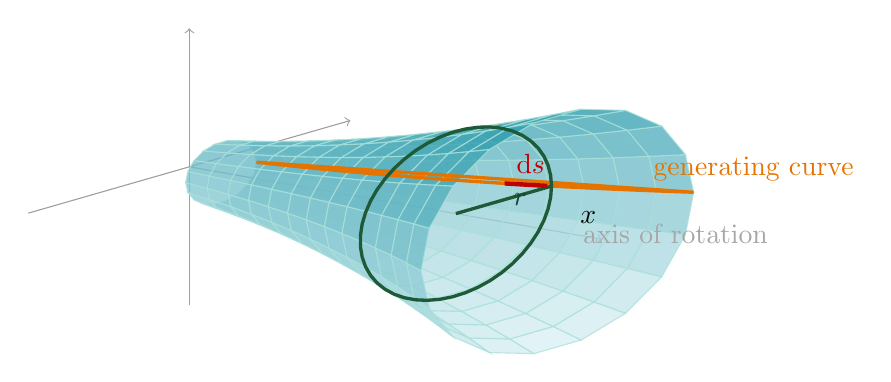
\begin{tikzpicture}
        \begin{axis}[
            width=0.9\textwidth,
            height=7.2cm,
            view={38}{23},
            axis lines=center,
            axis line style={->,gray!75},
            ticks=none,
            xlabel={\(x\)},
            xmin=0,
            xmax=6.5,
            ymin=-2.35,
            ymax=2.35,
            zmin=-2.35,
            zmax=2.35,
            enlargelimits=false,
            clip=false,
            colormap={surfaceblue}{
                rgb255(0cm)=(221,242,245);
                rgb255(1cm)=(35,151,169)
            }
        ]
            % The actual parametric surface
            % (x,f(x)cos(theta),f(x)sin(theta)).
            \addplot3[
                surf,
                shader=flat,
                opacity=0.78,
                draw=TealBlue!38,
                z buffer=sort,
                domain=0.5:5.8,
                y domain=0:360,
                samples=14,
                samples y=19
            ]
            ({x},
             {(0.45+0.12*x+0.025*x^2)*cos(y)},
             {(0.45+0.12*x+0.025*x^2)*sin(y)});

            % The generating curve before rotation.
            \addplot3[
                very thick,
                orange!90!black,
                domain=0.5:5.8,
                samples=40
            ]
            ({x},{0.45+0.12*x+0.025*x^2},{0});

            % One circular cross-section and its radius.
            \addplot3[
                very thick,
                SeaGreen!65!black,
                z buffer=none,
                domain=0:360,
                samples=48
            ]
            ({4.2},{(0.45+0.12*4.2+0.025*4.2^2)*cos(x)},
                   {(0.45+0.12*4.2+0.025*4.2^2)*sin(x)});
            \addplot3[very thick,SeaGreen!65!black]
                coordinates {(4.2,0,0) (4.2,1.395,0)};

            % A short arc-length element on the generating curve.
            \addplot3[ultra thick,red!75!black]
                coordinates {(3.65,1.2206,0) (4.15,1.3781,0)};

            \node[orange!90!black,anchor=south west]
                at (axis cs:5.25,1.77,0) {generating curve};
            \node[SeaGreen!50!black,anchor=west]
                at (axis cs:4.2,0.7,0) {\(r\)};
            \node[red!75!black,anchor=south]
                at (axis cs:3.9,1.37,0) {\(\mathrm{d}s\)};
            \node[gray!70,anchor=west]
                at (axis cs:6.05,0,0) {axis of rotation};
        \end{axis}
    \end{tikzpicture}
    \caption{A curve revolved about the \(x\)-axis.  At each point, a small
    arc of length \(\mathrm{d}s\) travels around a circle of radius \(r\),
    sweeping out a narrow band of area approximately
    \(2\pi r\,\mathrm{d}s\).}
    \label{fig:surface-of-revolution}
\end{figure}

\subsection{Derivation of the Formula}

Let \(f(x)\geq0\) and suppose that \(f'\) is continuous on \([a,b]\).
Choose a partition
\[
    P:\qquad a=x_0<x_1<\cdots<x_n=b
\]
and replace the graph of \(f\) by the polygonal path through the points
\[
    P_i=(x_i,y_i),
    \qquad y_i=f(x_i).
\]

For each \(i\), join \(P_{i-1}\) to \(P_i\) by a straight chord and denote
its length by
\[
    c_i=\lVert P_i-P_{i-1}\rVert.
\]
When this chord is revolved about the \(x\)-axis, it generates one conical
frustum.  Let \(A_i\) be the lateral area of that frustum and define
\[
    A(P)=\sum_{i=1}^n A_i.
\]
Thus \(A(P)\) is the area of the polygonal surface made from all the
frusta.  The surface area of the smooth surface is obtained by refining the
partition:
\[
    S=\lim_{\lVert P\rVert\to0}A(P),
    \qquad
    \lVert P\rVert
    =\max_{1\leq i\leq n}\Delta x_i,
    \qquad
    \Delta x_i=x_i-x_{i-1}.
\]
The calculation below proves that this limit exists and identifies it as an
integral.  Notice that the approximation is built from straight chords,
not from the original curved pieces.  Each piece in
Figure~\ref{fig:surface-partition-frusta} is a truncated cone between two
nearby circular cross-sections.

\begin{figure}[H]
    \centering
    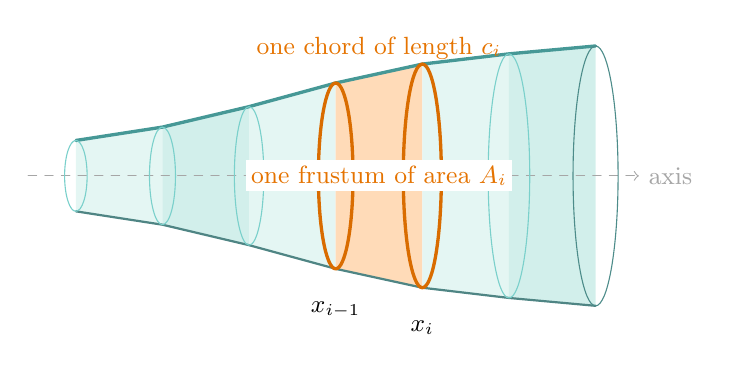
\begin{tikzpicture}[
        x=1.1cm,
        y=1cm,
        line cap=round,
        line join=round,
        every node/.style={font=\small}
    ]
        % Six adjacent frusta produced by six chords of the polygonal curve.
        \fill[TealBlue!12]
            (0.7,0.45)--(1.7,0.62)--(1.7,-0.62)--(0.7,-0.45)--cycle;
        \fill[TealBlue!20]
            (1.7,0.62)--(2.7,0.88)--(2.7,-0.88)--(1.7,-0.62)--cycle;
        \fill[TealBlue!12]
            (2.7,0.88)--(3.7,1.18)--(3.7,-1.18)--(2.7,-0.88)--cycle;
        \fill[orange!28]
            (3.7,1.18)--(4.7,1.42)--(4.7,-1.42)--(3.7,-1.18)--cycle;
        \fill[TealBlue!12]
            (4.7,1.42)--(5.7,1.55)--(5.7,-1.55)--(4.7,-1.42)--cycle;
        \fill[TealBlue!20]
            (5.7,1.55)--(6.7,1.65)--(6.7,-1.65)--(5.7,-1.55)--cycle;

        \draw[very thick,TealBlue!75!black]
            (0.7,0.45)--(1.7,0.62)--(2.7,0.88)--(3.7,1.18)--
            (4.7,1.42)--(5.7,1.55)--(6.7,1.65);
        \draw[thick,TealBlue!60!black]
            (0.7,-0.45)--(1.7,-0.62)--(2.7,-0.88)--(3.7,-1.18)--
            (4.7,-1.42)--(5.7,-1.55)--(6.7,-1.65);
        \draw[->,dashed,gray!70] (0.15,0)--(7.2,0)
            node[right] {axis};

        % The shared circular boundaries of the frusta.
        \draw[TealBlue!60] (0.7,0) ellipse (0.13 and 0.45);
        \draw[TealBlue!60] (1.7,0) ellipse (0.15 and 0.62);
        \draw[TealBlue!60] (2.7,0) ellipse (0.17 and 0.88);
        \draw[very thick,orange!85!black]
            (3.7,0) ellipse (0.20 and 1.18);
        \draw[very thick,orange!85!black]
            (4.7,0) ellipse (0.22 and 1.42);
        \draw[TealBlue!60] (5.7,0) ellipse (0.24 and 1.55);
        \draw[TealBlue!65!black] (6.7,0) ellipse (0.26 and 1.65);

        \node[above,orange!90!black] at (4.2,1.36)
            {one chord of length \(c_i\)};
        \node[orange!90!black,fill=white,inner sep=2pt]
            at (4.2,0) {one frustum of area \(A_i\)};
        \node[below] at (3.7,-1.48) {\(x_{i-1}\)};
        \node[below] at (4.7,-1.72) {\(x_i\)};
    \end{tikzpicture}
    \caption{The polygonal curve produces many adjacent conical frusta.
    Their circular edges match, so the sum
    \(A(P)=A_1+\cdots+A_n\) approximates the entire surface area.}
    \label{fig:surface-partition-frusta}
\end{figure}

The notation used in the proof has the following fixed meaning:
\[
    \begin{array}{ccl}
        P_i&=&\text{a point on the original graph},\\
        c_i&=&\text{the straight chord length from }P_{i-1}\text{ to }P_i,\\
        A_i&=&\text{the lateral area of the frustum generated by that chord},\\
        A(P)&=&\displaystyle\sum_{i=1}^n A_i,
                \text{ the polygonal surface area},\\
        S&=&\displaystyle\lim_{\lVert P\rVert\to0}A(P),
             \text{ the smooth surface area}.
    \end{array}
\]

\paragraph{Step 1: the exact area of one frustum.}
For the \(i\)-th chord, let
\[
    r_{i-1}=f(x_{i-1}),
    \qquad
    r_i=f(x_i),
\]
The two radii are \(r_{i-1}\) and \(r_i\), while the slant height is the
chord length \(c_i\).  Therefore the exact lateral area is
\[
    A_i=\pi(r_{i-1}+r_i)c_i.
\]
This formula can be derived from the lateral area \(\pi r\ell\) of a cone.
For example, suppose \(r_i>r_{i-1}\).  Extend the sloping sides of the
frustum until they meet at the apex of a cone.  If \(L_i\) and \(L_{i-1}\)
are the slant heights from the apex to the two circular edges, similarity of
triangles gives
\[
    \frac{L_i}{r_i}=\frac{L_{i-1}}{r_{i-1}},
    \qquad
    L_i-L_{i-1}=c_i.
\]

\begin{figure}[H]
    \centering
    \begin{tikzpicture}[
        x=1.05cm,
        y=1.05cm,
        line cap=round,
        line join=round,
        every node/.style={font=\small}
    ]
        \coordinate (O) at (0,0);
        \coordinate (D) at (3.6,1.44);
        \coordinate (E) at (3.6,-1.44);
        \coordinate (B) at (6,2.4);
        \coordinate (C) at (6,-2.4);
        \coordinate (Msmall) at (3.6,0);
        \coordinate (Mlarge) at (6,0);

        % The complete cone and the highlighted frustum.
        \fill[gray!8] (O)--(B)--(C)--cycle;
        \fill[orange!20] (D)--(B)--(C)--(E)--cycle;
        \draw[thick,TealBlue!70!black] (O)--(B);
        \draw[thick,TealBlue!70!black] (O)--(C);
        \draw[TealBlue!65!black] (Mlarge) ellipse (0.33 and 2.4);
        \draw[orange!85!black] (Msmall) ellipse (0.23 and 1.44);
        \draw[dashed,gray!70] (O)--(6.65,0) node[right] {axis};

        % Radii of the two circular cross-sections.
        \draw[<->,SeaGreen!65!black] (Msmall)--(D)
            node[midway,left] {\(r_{i-1}\)};
        \draw[<->,SeaGreen!65!black] (Mlarge)--(B)
            node[midway,right] {\(r_i\)};

        % Slant lengths: the upper side is split into L_{i-1} and c_i.
        \draw[very thick,orange!90!black] (D)--(B);
        \node[above,orange!90!black] at ($(D)!0.5!(B)$)
            {\(c_i=L_i-L_{i-1}\)};
        \node[above left,TealBlue!75!black] at ($(O)!0.55!(D)$)
            {\(L_{i-1}\)};
        \node[below left,TealBlue!75!black] at ($(O)!0.55!(C)$)
            {\(L_i\)};

        \fill (O) circle (1.4pt);
        \node[left] at (O) {apex};
        \node[orange!85!black] at (4.85,-0.45) {frustum};

        % Similar right triangles used in the proportion.
        \draw[gray!55]
            ($(Msmall)+(-0.14,0)$)--($(Msmall)+(-0.14,0.14)$)--
            ($(Msmall)+(0,0.14)$);
        \draw[gray!55]
            ($(Mlarge)+(-0.14,0)$)--($(Mlarge)+(-0.14,0.14)$)--
            ($(Mlarge)+(0,0.14)$);
    \end{tikzpicture}
    \caption{An axial cross-section of the frustum extended to a common
    apex.  The small and large right triangles are similar, so their slant
    heights and radii are proportional.  The frustum's slant height is the
    difference \(c_i=L_i-L_{i-1}\).}
    \label{fig:frustum-similar-triangles}
\end{figure}

Solving these equations yields
\[
    L_i=\frac{r_ic_i}{r_i-r_{i-1}},
    \qquad
    L_{i-1}=\frac{r_{i-1}c_i}{r_i-r_{i-1}}.
\]
The frustum is the large cone with the small cone removed, so
\begin{align*}
    A_i
    &=\pi r_iL_i-\pi r_{i-1}L_{i-1} \\
    &=\pi c_i
      \frac{r_i^2-r_{i-1}^2}{r_i-r_{i-1}} \\
    &=\pi(r_i+r_{i-1})c_i.
\end{align*}
The same result holds if \(r_i<r_{i-1}\).  If the radii are equal, the
frustum is a cylinder and the formula reduces to
\(2\pi r_ic_i\), as expected.  Equivalently,
\[
    \overline r_i=\frac{r_{i-1}+r_i}{2},
    \qquad
    A_i=2\pi\overline r_i c_i.
\]
Thus the area of one frustum is exactly
\[
    \underbrace{2\pi\overline r_i}_{\text{circumference at average radius}}
    \times
    \underbrace{c_i}_{\text{chord length}}.
\]

\begin{figure}[H]
    \centering
    \begin{tikzpicture}[
        x=1.15cm,
        y=1.05cm,
        line cap=round,
        line join=round,
        every node/.style={font=\small}
    ]
        \coordinate (Ltop) at (1.2,1.05);
        \coordinate (Lbottom) at (1.2,-1.05);
        \coordinate (Rtop) at (5.4,1.75);
        \coordinate (Rbottom) at (5.4,-1.75);

        % The local chord sweeps out this conical frustum.
        \fill[orange!18]
            (Ltop)--(Rtop)--(Rbottom)--(Lbottom)--cycle;
        \draw[very thick,orange!85!black] (Ltop)--(Rtop);
        \draw[thick,orange!70!black] (Lbottom)--(Rbottom);
        \draw[TealBlue!70!black] (1.2,0) ellipse (0.24 and 1.05);
        \draw[TealBlue!70!black] (5.4,0) ellipse (0.38 and 1.75);
        \draw[dashed,gray!75] (0.45,0)--(6.15,0);

        % Radii and slant height used in the frustum-area formula.
        \draw[<->,SeaGreen!65!black] (1.2,0)--(Ltop)
            node[midway,left] {\(r_{i-1}\)};
        \draw[<->,SeaGreen!65!black] (5.4,0)--(Rtop)
            node[midway,right] {\(r_i\)};
        \node[above,orange!90!black]
            at ($(Ltop)!0.5!(Rtop)$) {\(c_i\)};

        \node[below] at (1.2,-1.35) {at \(x_{i-1}\)};
        \node[below] at (5.4,-2.05) {at \(x_i\)};
        \node[gray!75,anchor=west] at (5.72,0.15)
            {axis};
    \end{tikzpicture}
    \caption{A short chord produces a conical frustum.  Its lateral area is
    \(\pi(r_{i-1}+r_i)c_i\), or circumference at the average radius
    times slant height.}
    \label{fig:surface-area-frustum}
\end{figure}

\paragraph{Step 2: express the chord length in terms of \(f'\).}
Set
\[
    \Delta x_i=x_i-x_{i-1},
    \qquad
    \Delta y_i=f(x_i)-f(x_{i-1}).
\]
The slant height of the frustum is exactly the length of the chord, so the
Pythagorean theorem gives
\begin{align*}
    c_i
    &=\sqrt{(\Delta x_i)^2+(\Delta y_i)^2} \\
    &=\sqrt{1+\left(\frac{\Delta y_i}{\Delta x_i}\right)^2}
      \,\Delta x_i.
\end{align*}
Because \(f\) is continuous on \([x_{i-1},x_i]\) and differentiable in its
interior, the Mean Value Theorem supplies a point
\(\xi_i\in(x_{i-1},x_i)\) such that
\[
    \frac{\Delta y_i}{\Delta x_i}=f'(\xi_i).
\]
Therefore,
\[
    c_i
    =\sqrt{1+\bigl(f'(\xi_i)\bigr)^2}\,\Delta x_i.
\]
This is an exact formula for the chord length.  It does not assert that
\(c_i\) is the length of the curved portion of the graph.  At this stage we
are computing the area of the polygonal approximation, so only the straight
chord is needed.
Substituting this into the exact frustum formula gives
\[
    A_i
    =2\pi
      \left(\frac{f(x_{i-1})+f(x_i)}{2}\right)
      \sqrt{1+\bigl(f'(\xi_i)\bigr)^2}\,\Delta x_i.
\]
Hence the area of the entire polygonal surface is
\[
    A(P)=2\pi\sum_{i=1}^n
      \left(\frac{f(x_{i-1})+f(x_i)}{2}\right)
      \sqrt{1+\bigl(f'(\xi_i)\bigr)^2}\,\Delta x_i.
\]

\paragraph{Step 3: pass from the sum to an integral.}
The only remaining issue is the radius.  The exact frustum formula uses the
average endpoint radius
\[
    \overline r_i=\frac{f(x_{i-1})+f(x_i)}{2},
\]
whereas a standard Riemann sum evaluates every factor at one sample point.
On a very short subinterval, however, \(f(x_{i-1})\), \(f(\xi_i)\), and
\(f(x_i)\) are all close.  Therefore \(\overline r_i\) may be replaced by
\(f(\xi_i)\) in the limit.  The following estimate makes this precise.

Define
\[
    q(x)=\sqrt{1+\bigl(f'(x)\bigr)^2}.
\]
Since \(f'\) is continuous on the closed interval \([a,b]\), both \(q\)
and
\[
    f(x)q(x)=f(x)\sqrt{1+\bigl(f'(x)\bigr)^2}
\]
are continuous and therefore Riemann integrable.  If the average radius in
the preceding sum were replaced by \(f(\xi_i)\), we would obtain the
ordinary Riemann sum
\[
    2\pi\sum_{i=1}^n
    f(\xi_i)q(\xi_i)\,\Delta x_i,
\]
which converges to
\[
    2\pi\int_a^b f(x)q(x)\,\mathrm{d}x.
\]

It remains to justify replacing the average endpoint radius by
\(f(\xi_i)\).  Because \(f\) is continuous on the compact interval
\([a,b]\), it is uniformly continuous.  Let
\[
    \omega_f(\delta)
    =\sup\{\lvert f(u)-f(v)\rvert:
            u,v\in[a,b],\ \lvert u-v\rvert\leq\delta\}
\]
be its modulus of continuity.  Since \(x_{i-1}\), \(\xi_i\), and \(x_i\)
all lie in an interval of width at most \(\lVert P\rVert\),
\[
    \left\lvert
        \frac{f(x_{i-1})+f(x_i)}{2}-f(\xi_i)
    \right\rvert
    \leq\omega_f(\lVert P\rVert).
\]
Also, \(q\) is continuous on \([a,b]\), so it has a finite maximum \(M\).
The difference between the frustum sum and the ordinary Riemann sum is thus
at most
\begin{align*}
    &2\pi\sum_{i=1}^n
      \omega_f(\lVert P\rVert)M\,\Delta x_i \\
    &\qquad=2\pi M(b-a)\omega_f(\lVert P\rVert),
\end{align*}
which approaches \(0\) as \(\lVert P\rVert\to0\).  Consequently,
\begin{align*}
    S
    &=\lim_{\lVert P\rVert\to0}A(P) \\
    &=2\pi\int_a^b
      f(x)\sqrt{1+\bigl(f'(x)\bigr)^2}\,\mathrm{d}x.
\end{align*}

Only after taking this limit do we introduce the arc-length differential
\(\mathrm{d}s\).  It abbreviates the limiting factor
\[
    \mathrm{d}s
    =\sqrt{1+\bigl(f'(x)\bigr)^2}\,\mathrm{d}x.
\]
Thus the final formula is often remembered symbolically as
\[
    \mathrm{d}S=2\pi f(x)\,\mathrm{d}s.
\]
This notation describes the limiting integral.  It does not say that the
finite chord length \(c_i\) is equal to the length of the corresponding
curved piece.  Geometrically, it says that an infinitesimally narrow surface
band has area equal to its circumference \(2\pi f(x)\) times its
infinitesimal slant width \(\mathrm{d}s\).

\begin{theorem}[Surface area about the \(x\)-axis]
    Suppose \(f(x)\geq0\) and \(f'\) is continuous on \([a,b]\).  The area
    of the surface obtained by revolving \(y=f(x)\) about the \(x\)-axis is
    \[
        S=2\pi\int_a^b
        f(x)\sqrt{1+\bigl(f'(x)\bigr)^2}\,\mathrm{d}x.
    \]
    If \(f\) may be negative, replace \(f(x)\) by \(\lvert f(x)\rvert\),
    since the radius is a distance and must be nonnegative.
\end{theorem}

The two factors in the integrand have clear geometric meanings:
\[
    \underbrace{2\pi f(x)}_{\text{circumference}}
    \underbrace{\sqrt{1+\bigl(f'(x)\bigr)^2}\,\mathrm{d}x}
                _{\text{arc-length element}}.
\]
Using only \(2\pi f(x)\,\mathrm{d}x\) would treat the sloping piece of the
curve as horizontal and would therefore underestimate its surface area.

\subsection{Rotation about the \(y\)-Axis}

When \(y=f(x)\) is revolved about the \(y\)-axis, the radius is the distance
from the point \((x,f(x))\) to that axis.  If \(0\leq a<b\), then \(r=x\),
and hence
\[
    S=2\pi\int_a^b
    x\sqrt{1+\bigl(f'(x)\bigr)^2}\,\mathrm{d}x.
\]
More generally, if the interval includes negative values of \(x\), the
radius is \(\lvert x\rvert\).  Care must also be taken to avoid counting the
same surface more than once if different parts of the curve trace the same
surface after rotation.

If the curve is written as \(x=g(y)\), where \(g'\) is continuous for
\(c\leq y\leq d\), then
\[
    \mathrm{d}s=\sqrt{1+\bigl(g'(y)\bigr)^2}\,\mathrm{d}y.
\]
Consequently,
\[
    \begin{aligned}
        \text{about the \(y\)-axis:}\qquad
        S&=2\pi\int_c^d
        \lvert g(y)\rvert\sqrt{1+\bigl(g'(y)\bigr)^2}\,\mathrm{d}y,\\
        \text{about the \(x\)-axis:}\qquad
        S&=2\pi\int_c^d
        \lvert y\rvert\sqrt{1+\bigl(g'(y)\bigr)^2}\,\mathrm{d}y.
    \end{aligned}
\]

\subsection{Parametric Form}

For a parametrized curve
\[
    x=x(t),\qquad y=y(t),\qquad \alpha\leq t\leq\beta,
\]
the arc-length element is
\[
    \mathrm{d}s
    =\sqrt{\bigl(x'(t)\bigr)^2+\bigl(y'(t)\bigr)^2}\,\mathrm{d}t.
\]
Therefore, provided the surface is traced only once,
\[
    \begin{aligned}
        \text{about the \(x\)-axis:}\qquad
        S&=2\pi\int_\alpha^\beta
        \lvert y(t)\rvert
        \sqrt{\bigl(x'(t)\bigr)^2+\bigl(y'(t)\bigr)^2}\,\mathrm{d}t,\\
        \text{about the \(y\)-axis:}\qquad
        S&=2\pi\int_\alpha^\beta
        \lvert x(t)\rvert
        \sqrt{\bigl(x'(t)\bigr)^2+\bigl(y'(t)\bigr)^2}\,\mathrm{d}t.
    \end{aligned}
\]
In every form, the same principle is being used:
\[
    \boxed{\mathrm{d}S=(\text{circumference})\,\mathrm{d}s
    =2\pi(\text{radius})\,\mathrm{d}s.}
\]

\section{Differential Equations}

A \emph{differential equation} is an equation involving an unknown function
and one or more of its derivatives.  Its \emph{order} is the order of the
highest derivative that occurs.  For example,
\[
    y'=x-y
    \qquad\text{and}\qquad
    y''+4y=0
\]
are first- and second-order differential equations, respectively.  A
function is a solution on an interval only if it satisfies the equation at
every point of that interval.

Most problems in elementary calculus are \emph{initial-value problems}:
the differential equation is accompanied by enough values of the unknown
function and its derivatives to determine the arbitrary constants.  A
first-order equation normally requires one condition, such as
\(y(x_0)=y_0\), whereas a second-order equation normally requires two, such
as \(y(x_0)=y_0\) and \(y'(x_0)=v_0\).

\subsection{First-Order Differential Equations}

A general first-order equation has the form
\[
    F(x,y,y')=0.
\]
There is no single method that solves every such equation.  The important
first step is therefore to recognize its form.

\subsubsection{Direction fields and Euler's method}

If the equation can be written as
\[
    y'=f(x,y),
\]
then the number \(f(x,y)\) gives the slope of a solution curve through the
point \((x,y)\).  Drawing a short segment with this slope at many points
produces a \emph{direction field}.  Even when an exact formula is
unavailable, the field reveals whether solutions increase or decrease,
where equilibrium solutions occur, and how solutions behave in the long
run.

Euler's method replaces the solution curve by short tangent-line steps.
Starting with \((x_0,y_0)\) and using a step size \(h\), define
\[
    x_{n+1}=x_n+h,
    \qquad
    y_{n+1}=y_n+h f(x_n,y_n).
\]
The approximation \(y_n\approx y(x_n)\) is usually improved by choosing a
smaller \(h\), although more steps are then required.

The geometry of one Euler step is especially simple.  At the current
approximation \(P_n=(x_n,y_n)\), the differential equation prescribes the
slope \(f(x_n,y_n)\).  Moving horizontally by \(h\) along the corresponding
tangent line changes the height by
\[
    \Delta y=(\text{slope})(\text{horizontal change})
             =h f(x_n,y_n).
\]
Thus the endpoint of that tangent-line segment is precisely
\(P_{n+1}=(x_n+h,y_n+h f(x_n,y_n))\).

\begin{figure}[H]
    \centering
    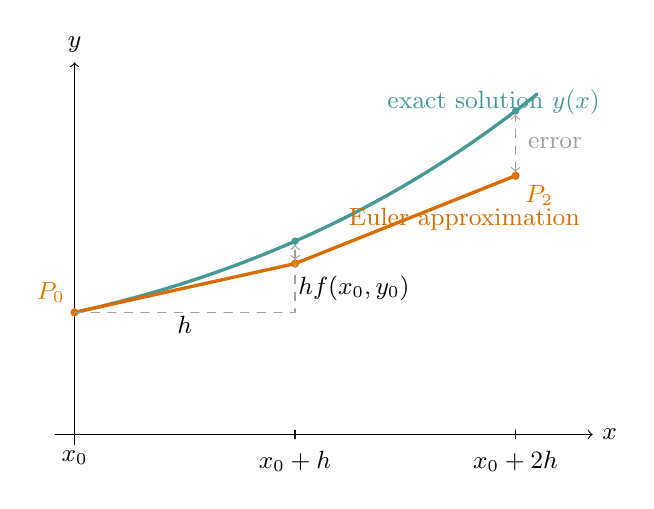
\begin{tikzpicture}[
        x=7cm,
        y=1.55cm,
        line cap=round,
        line join=round,
        every node/.style={font=\small}
    ]
        % Axes.
        \draw[->] (-0.035,0)--(0.94,0) node[right] {\(x\)};
        \draw[->] (0,-0.08)--(0,3.05) node[above] {\(y\)};

        % The exact solution y=2e^x-x-1 of y'=x+y, y(0)=1.
        \draw[very thick,TealBlue!75!black]
            plot[smooth,samples=80,domain=0:0.84]
            (\x,{2*exp(\x)-\x-1});
        \node[TealBlue!75!black,anchor=west]
            at (0.55,2.72) {exact solution \(y(x)\)};

        % Euler polygon for h=0.4: (0,1), (0.4,1.4), (0.8,2.12).
        \draw[very thick,orange!85!black]
            (0,1)--(0.4,1.4)--(0.8,2.12);
        \fill[orange!90!black] (0,1) circle[radius=1.5pt]
            node[above left] {\(P_0\)};
        \fill[orange!90!black] (0.4,1.4) circle[radius=1.5pt]
            node[below right] {\(P_1\)};
        \fill[orange!90!black] (0.8,2.12) circle[radius=1.5pt]
            node[below right] {\(P_2\)};
        \node[orange!85!black,anchor=west]
            at (0.48,1.76) {Euler approximation};

        % Slope triangle for the first Euler step.
        \draw[dashed,gray!75] (0,1)--(0.4,1)--(0.4,1.4);
        \node[below,fill=white,inner sep=1pt] at (0.2,1)
            {\(h\)};
        \node[right,fill=white,inner sep=1pt] at (0.4,1.2)
            {\(h f(x_0,y_0)\)};

        % Exact values at the mesh points and the accumulated errors.
        \fill[TealBlue!75!black] (0.4,1.58365) circle[radius=1.35pt];
        \fill[TealBlue!75!black] (0.8,2.65108) circle[radius=1.35pt];
        \draw[<->,dashed,gray!75]
            (0.4,1.43)--(0.4,1.55365);
        \draw[<->,dashed,gray!75]
            (0.8,2.15)--(0.8,2.62108);
        \node[gray!75,anchor=west] at (0.805,2.39) {error};

        % Mesh marks.
        \draw (0,-0.035)--(0,0.035) node[below=4pt] {\(x_0\)};
        \draw (0.4,-0.035)--(0.4,0.035) node[below=4pt] {\(x_0+h\)};
        \draw (0.8,-0.035)--(0.8,0.035) node[below=4pt] {\(x_0+2h\)};
    \end{tikzpicture}
    \caption{Euler's method follows a tangent line for one short horizontal
    step and then recomputes the slope.  The illustration uses
    \(y'=x+y\), \(y(0)=1\), and \(h=0.4\); the larger step size makes the
    approximation error visible.}
    \label{fig:eulers-method}
\end{figure}

The orange segment from \(P_0\) uses the slope at \(P_0\).  At \(P_1\),
Euler's method discards the old slope and uses the new slope
\(f(x_1,y_1)\) for the next segment.  Notice that \(P_1\) is generally not
on the exact solution.  Consequently, the next slope is also evaluated at
an approximate point, so the error can accumulate from one step to the
next.  A smaller step size keeps each tangent-line segment closer to the
curved solution.

\begin{eg}[Euler approximation]
    For
    \[
        y'=x+y,
        \qquad y(0)=1,
    \]
    use \(h=0.1\).  Since \(f(x,y)=x+y\),
    \[
        y_1=1+0.1f(0,1)=1.1.
    \]
    The next step gives
    \[
        y_2=1.1+0.1f(0.1,1.1)=1.22.
    \]
    Thus Euler's method gives \(y(0.2)\approx1.22\).
\end{eg}

\subsubsection{Separable equations}

An equation is \emph{separable} if it can be written in the form
\[
    \frac{\mathrm{d}y}{\mathrm{d}x}=g(x)h(y).
\]
When \(h(y)\neq0\), place all factors involving \(y\) with
\(\mathrm{d}y\), place all factors involving \(x\) with
\(\mathrm{d}x\), and integrate:
\[
    \frac{1}{h(y)}\,\mathrm{d}y=g(x)\,\mathrm{d}x,
    \qquad
    \int\frac{1}{h(y)}\,\mathrm{d}y
    =\int g(x)\,\mathrm{d}x+C.
\]
The result may define \(y\) implicitly.  Before dividing by \(h(y)\), one
must separately check the constant solutions obtained from \(h(y)=0\).

\begin{eg}[A separable initial-value problem]
    Solve
    \[
        y'=xy,
        \qquad y(0)=3.
    \]
    For a nonzero solution,
    \[
        \frac{1}{y}\,\mathrm{d}y=x\,\mathrm{d}x.
    \]
    Integration gives
    \[
        \ln|y| = \frac{x^2}{2} + C^{\prime} ,
    \]
    so \(y=Ce^{x^2/2}\), where the new constant \(C\) may be positive or
    negative.  The initial condition yields \(C=3\).  Therefore,
    \[
        \boxed{y=3e^{x^2/2}}.
    \]
    The constant solution \(y=0\), lost when we divided by \(y\), also
    solves the differential equation but not the given initial condition.
\end{eg}

Two common models are immediate examples of separation.  Exponential
growth or decay satisfies
\[
    \frac{\mathrm{d}P}{\mathrm{d}t}=kP,
    \qquad
    P(t)=P_0e^{kt}.
\]
Logistic growth satisfies
\[
    \frac{\mathrm{d}P}{\mathrm{d}t}
    =kP\left(1-\frac{P}{K}\right),
\]
where \(K>0\) is the carrying capacity.  If \(P(0)=P_0>0\), then
\[
    P(t)=\frac{K}{1+Ae^{-kt}},
    \qquad
    A=\frac{K-P_0}{P_0}.
\]

\subsubsection{First-order linear equations}

A first-order equation is \emph{linear} if it can be put into standard form
\[
    y'+P(x)y=Q(x).
\]
Its integrating factor is
\[
    \mu(x)=e^{\int P(x)\,\mathrm{d}x}.
\]
Multiplying the entire equation by \(\mu\) makes the left-hand side a
product derivative:
\[
    \mu y'+\mu Py=(\mu y)'=\mu Q.
\]
Consequently,
\[
    \mu(x)y(x)=\int\mu(x)Q(x)\,\mathrm{d}x+C,
\]
or
\[
    \boxed{
        y(x)=\frac{1}{\mu(x)}
        \left(\int\mu(x)Q(x)\,\mathrm{d}x+C\right).}
\]
Multiplying the equation by a nonzero constant multiple of \(\mu\) gives
the same family of solutions.

\begin{eg}[The integrating-factor method]
    Solve
    \[
        y'+2y=e^x,
        \qquad y(0)=1.
    \]
    Here \(P(x)=2\), so \(\mu(x)=e^{2x}\).  Multiplication gives
    \[
        e^{2x}y'+2e^{2x}y=e^{3x},
        \qquad
        (e^{2x}y)'=e^{3x}.
    \]
    Hence
    \[
        e^{2x}y=\frac13e^{3x}+C,
        \qquad
        y=\frac13e^x+Ce^{-2x}.
    \]
    From \(y(0)=1\), we obtain \(C=2/3\), and therefore
    \[
        \boxed{y=\frac13e^x+\frac23e^{-2x}}.
    \]
\end{eg}

\begin{remark}[Choosing a first-order method]
    First simplify the equation and ask the following questions.
    \begin{enumerate}
        \item Can it be written as \(y'=g(x)h(y)\)?  If so, separate the
        variables.
        \item Can it be written as \(y'+P(x)y=Q(x)\)?  If so, use an
        integrating factor.
        \item If neither form applies, use a direction field or a numerical
        method to study the solution.  Some equations require techniques
        beyond a first calculus course.
    \end{enumerate}
    An equation may be both separable and linear; either valid method may be
    used.
\end{remark}

\subsection{Second-Order Differential Equations}

A general second-order equation has the form
\[
    F(x,y,y',y'')=0.
\]
The main class treated in introductory calculus is the linear equation
\[
    a(x)y''+b(x)y'+c(x)y=g(x).
\]
It is \emph{homogeneous} when \(g(x)=0\) and \emph{nonhomogeneous} when
\(g(x)\neq0\).  The word homogeneous here refers to the right-hand side;
it does not mean that all coefficients are constant.

\subsubsection{Equations that can be reduced in order}

Some second-order equations contain only one of the variables \(x\) and
\(y\).  Their missing variable indicates a useful substitution that turns
the equation into a first-order equation.  After solving that first-order
equation, one more integration recovers \(y\).  This process is called
\emph{reduction of order}.

\paragraph{Case 1: the dependent variable \(y\) is missing.}
Suppose the equation has the form
\[
    F(x,y',y'')=0.
\]
Because only derivatives of \(y\) occur, define a new unknown function
\[
    v(x)=y'(x).
\]
Since \(v\) is a function of \(x\),
\[
    v'(x)=y''(x).
\]
The original second-order equation therefore becomes the first-order
equation
\[
    F(x,v,v')=0.
\]
The solution proceeds in two stages:
\[
    \boxed{
        \text{solve for \(v\)}
        \quad\longrightarrow\quad
        \text{solve \(y'=v(x)\) for \(y\)}.}
\]
The first stage introduces one constant, and the final integration normally
introduces a second constant.

\begin{eg}[When \(y\) is missing]
    Solve the initial-value problem
    \[
        y''+3y'=0,
        \qquad y(0)=2,
        \qquad y'(0)=6.
    \]
    Set \(v=y'\), so that \(v'=y''\).  The equation becomes
    \[
        v'+3v=0.
    \]
    This first-order equation is separable:
    \[
        \frac{\mathrm{d}v}{v}=-3\,\mathrm{d}x,
        \qquad
        v=Ce^{-3x}.
    \]
    Since \(v(0)=y'(0)=6\), we have \(C=6\).  We have now found the
    derivative, not yet the original function:
    \[
        y'=v=6e^{-3x}.
    \]
    Integrating once more gives
    \[
        y=-2e^{-3x}+D.
    \]
    Finally, \(y(0)=2\) implies \(D=4\).  Hence
    \[
        \boxed{y=4-2e^{-3x}}.
    \]
    Indeed, \(y'=6e^{-3x}\) and \(y''=-18e^{-3x}\), so
    \(y''+3y'=0\).
\end{eg}

The especially simple equation \(y''=g(x)\) belongs to this case: integrate
once to find \(y'\), then integrate again to find \(y\).

\paragraph{Case 2: the independent variable \(x\) is missing.}
Now suppose the equation has the form
\[
    F(y,y',y'')=0.
\]
Here the substitution is different.  Regard \(y'=v\) as a function of
\(y\), rather than directly as a function of \(x\):
\[
    v(y)=y'.
\]
The chain rule is essential.  It gives
\[
    y''
    =\frac{\mathrm{d}}{\mathrm{d}x}\bigl(v(y)\bigr)
    =\frac{\mathrm{d}v}{\mathrm{d}y}
       \frac{\mathrm{d}y}{\mathrm{d}x}
    =v\frac{\mathrm{d}v}{\mathrm{d}y}.
\]
Thus make the replacements
\[
    \boxed{
        y'=v,
        \qquad
        y''=v\frac{\mathrm{d}v}{\mathrm{d}y}.}
\]
The result is a first-order equation whose independent variable is now
\(y\).  Solve it for \(v(y)\), and then solve the first-order equation
\[
    \frac{\mathrm{d}y}{\mathrm{d}x}=v(y)
\]
to recover \(y\) as a function of \(x\).

\begin{eg}[When \(x\) is missing]
    Solve
    \[
        yy''=(y')^2,
        \qquad y(0)=2,
        \qquad y'(0)=6.
    \]
    Set \(v(y)=y'\).  Since
    \(y''=v\,\mathrm{d}v/\mathrm{d}y\), the equation becomes
    \[
        yv\frac{\mathrm{d}v}{\mathrm{d}y}=v^2.
    \]
    The initial value \(v(2)=6\) is nonzero, so near the initial point we
    may divide by \(yv\):
    \[
        \frac{1}{v}\frac{\mathrm{d}v}{\mathrm{d}y}=\frac{1}{y}.
    \]
    Integrating with respect to \(y\) gives
    \[
        \ln|v|=\ln|y|+C,
        \qquad
        v=Ky.
    \]
    Since \(v(2)=6\), we obtain \(K=3\).  Returning to the original
    variables now gives a first-order equation:
    \[
        y'=v=3y.
    \]
    Its solution is \(y=Ae^{3x}\), and \(y(0)=2\) gives \(A=2\).
    Therefore,
    \[
        \boxed{y=2e^{3x}}.
    \]
\end{eg}

\begin{remark}[Two substitutions that must not be confused]
    When \(y\) is missing, use \(v(x)=y'\) and hence \(y''=v'\).  When
    \(x\) is missing, use \(v(y)=y'\) and hence
    \(y''=v\,\mathrm{d}v/\mathrm{d}y\).  Writing \(y''=v'\) in the second
    case without specifying the variable of differentiation loses the
    chain-rule factor \(v\).

    As with separable equations, check separately for solutions lost by
    division.  For example, dividing by \(v\) can discard the branch
    \(v=0\), which corresponds to constant solutions \(y'=0\).
\end{remark}

\subsubsection{Homogeneous equations with constant coefficients}

Consider
\[
    ay''+by'+cy=0,
    \qquad a\neq0,
\]
where \(a,b,c\) are real constants.  It is called \emph{homogeneous}
because its right-hand side is zero.  Before trying to solve it, we first
explain the structure of its set of solutions.

\begin{theorem}[Existence and uniqueness for the initial-value problem]
    Fix \(x_0\in\mathbb{R}\).  For every pair of real numbers \(A,B\), the
    problem
    \[
        ay''+by'+cy=0,
        \qquad
        y(x_0)=A,
        \qquad
        y'(x_0)=B
    \]
    has exactly one solution.
\end{theorem}
\begin{proof}
    Divide the equation by \(a\) and write it as
    \[
        y''=p y'+q y,
        \qquad
        p=-\frac{b}{a},
        \qquad
        q=-\frac{c}{a}.
    \]
    We prove existence and uniqueness separately, without using the
    characteristic-root formulas that will be derived later.

    \begin{subproof}[Existence]
        Seek a power-series solution centered at \(x_0\):
        \[
            y(x)=\sum_{n=0}^{\infty}c_n(x-x_0)^n.
        \]
        The initial conditions require
        \[
            c_0=A,
            \qquad
            c_1=B.
        \]
        Formally differentiating gives
        \begin{align*}
            y'
            &=\sum_{n=0}^{\infty}(n+1)c_{n+1}(x-x_0)^n,\\
            y''
            &=\sum_{n=0}^{\infty}(n+2)(n+1)c_{n+2}(x-x_0)^n.
        \end{align*}
        Matching the coefficient of \((x-x_0)^n\) in
        \(y''=py'+qy\) gives the recurrence
        \[
            \boxed{
            (n+2)(n+1)c_{n+2}
            =p(n+1)c_{n+1}+q c_n.}
        \]
        Thus \(c_0=A\) and \(c_1=B\) determine \(c_2\), which determines
        \(c_3\), and so on.  There is therefore at most one power series
        with the prescribed initial values.

        We must verify that the resulting series actually converges.  Choose
        \(R\geq1\) large enough that
        \[
            R^2\geq |p|R+|q|,
        \]
        and let
        \[
            K=\max\left\{|A|,\frac{|B|}{R}\right\}.
        \]
        We claim that
        \[
            |c_n|\leq K\frac{R^n}{n!}
            \qquad(n\geq0).
        \]
        This is true for \(n=0,1\).  If it holds for \(n\) and \(n+1\),
        the recurrence gives
        \begin{align*}
            |c_{n+2}|
            &\leq
            \frac{|p|(n+1)|c_{n+1}|+|q||c_n|}
                 {(n+2)(n+1)}\\
            &\leq
            K\frac{R^n(|p|R+|q|)}{(n+2)!}\\
            &\leq K\frac{R^{n+2}}{(n+2)!}.
        \end{align*}
        Induction proves the claim.

        Consequently, for every real \(x\),
        \[
            \sum_{n=0}^{\infty}|c_n||x-x_0|^n
            \leq
            K\sum_{n=0}^{\infty}
            \frac{(R|x-x_0|)^n}{n!}
            =K e^{R|x-x_0|}.
        \]
        The series therefore converges for every \(x\).  The same estimate
        applied after one or two differentiations shows that the derivative
        series also converge on every bounded interval.  Hence the series
        may be differentiated twice term by term.  The recurrence then
        guarantees that the resulting function satisfies
        \(y''=py'+qy\), while \(c_0=A\) and \(c_1=B\) give the prescribed
        initial values.  A solution therefore exists.
    \end{subproof}

    \begin{subproof}[Uniqueness]
        Suppose \(y_1\) and \(y_2\) are two solutions with the same initial
        values, and set
        \[
            w=y_1-y_2.
        \]
        Then
        \[
            w''=pw'+qw,
            \qquad
            w(x_0)=w'(x_0)=0.
        \]
        Define the nonnegative function
        \[
            E(x)=w(x)^2+w'(x)^2.
        \]
        Using the differential equation,
        \begin{align*}
            E'
            &=2ww'+2w'w''\\
            &=2(1+q)ww'+2p(w')^2.
        \end{align*}
        Since \(2|ww'|\leq w^2+(w')^2=E\), there is a constant
        \[
            M=|1+q|+2|p|
        \]
        such that
        \[
            |E'(x)|\leq M E(x).
        \]

        For \(x\geq x_0\), the inequality \(E'\leq ME\) gives
        \[
            \frac{\mathrm{d}}{\mathrm{d}x}
            \bigl(e^{-Mx}E(x)\bigr)\leq0.
        \]
        Since \(E(x_0)=0\) and \(E\geq0\), this forces \(E(x)=0\) for
        \(x\geq x_0\).  For \(x\leq x_0\), the inequality
        \(E'\geq-ME\) similarly gives
        \[
            \frac{\mathrm{d}}{\mathrm{d}x}
            \bigl(e^{Mx}E(x)\bigr)\geq0,
        \]
        which again forces \(E(x)=0\).  Thus \(E\equiv0\), so
        \(w\equiv0\), and consequently \(y_1=y_2\).  The solution is
        unique.
    \end{subproof}
\end{proof}

The proof shows precisely why two initial values may be chosen freely:
they are the first two coefficients of the power series, and the
differential equation recursively determines every later coefficient.

\begin{theorem}[The solution space has dimension two]
    Let \(I\) be an interval containing \(x_0\), and let
    \[
        \mathcal{S}
        =\{y\in C^2(I,\mathbb{R}):ay''+by'+cy=0\}.
    \]
    Then \(\mathcal{S}\) is a two-dimensional real vector space.
\end{theorem}
\begin{proof}
    The zero function is a solution.  Moreover, if \(y_1,y_2\) are
    solutions and \(s,t\in\mathbb{R}\), then
    \begin{align*}
        a(sy_1+ty_2)''+b(sy_1+ty_2)'+c(sy_1+ty_2)
        &=s(ay_1''+by_1'+cy_1) \\
        &\quad+t(ay_2''+by_2'+cy_2) \\
        &=0.
    \end{align*}
    Thus every linear combination of solutions is again a solution, so
    \(\mathcal{S}\) is a vector space.

    Now assign to each solution its two initial values:
    \[
        \Phi:\mathcal{S}\longrightarrow\mathbb{R}^2,
        \qquad
        \Phi(y)=\bigl(y(x_0),y'(x_0)\bigr).
    \]
    This map is linear.  The existence part of the preceding theorem says
    that every pair \((A,B)\in\mathbb{R}^2\) is \(\Phi(y)\) for some
    solution \(y\), so \(\Phi\) is onto.  The uniqueness part says that two
    solutions with the same initial values must be identical, so \(\Phi\)
    is one-to-one.  Hence \(\Phi\) is a linear isomorphism
    \[
        \mathcal{S}\cong\mathbb{R}^2.
    \]
    Since \(\mathbb{R}^2\) has dimension \(2\), so does \(\mathcal{S}\).
\end{proof}

This theorem gives the central strategy.  We do not need to guess every
solution directly.  It is enough to find two solutions \(y_1,y_2\) that are
\emph{linearly independent}, meaning that
\[
    C_1y_1+C_2y_2=0
    \quad\text{as a function}
\]
is possible only when \(C_1=C_2=0\).  Two linearly independent vectors in
a two-dimensional vector space form a basis.  Therefore every solution is
then automatically of the form
\[
    \boxed{y=C_1y_1+C_2y_2.}
\]

\paragraph{Finding special solutions with an exponential.}
Exponential functions are useful because differentiation does not change
their basic form:
\[
    y=e^{rx},
    \qquad
    y'=re^{rx},
    \qquad
    y''=r^2e^{rx}.
\]
Substitution gives
\[
    ay''+by'+cy
    =(ar^2+br+c)e^{rx}.
\]
Because \(e^{rx}\neq0\), the function \(e^{rx}\) is a solution precisely
when \(r\) satisfies the \emph{characteristic equation}
\[
    ar^2+br+c=0.
\]
We now use its roots to find two independent special solutions.

\paragraph{Case 1: two distinct real roots.}
Suppose the characteristic roots are \(r_1\neq r_2\).  Then
\[
    y_1=e^{r_1x},
    \qquad
    y_2=e^{r_2x}
\]
are solutions.  To check independence, suppose
\[
    C_1e^{r_1x}+C_2e^{r_2x}=0
\]
for every \(x\).  Evaluating this equation and its derivative at \(x_0\)
gives
\[
    \begin{aligned}
        C_1e^{r_1x_0}+C_2e^{r_2x_0}&=0,\\
        r_1C_1e^{r_1x_0}+r_2C_2e^{r_2x_0}&=0.
    \end{aligned}
\]
Subtracting \(r_1\) times the first equation from the second gives
\[
    (r_2-r_1)C_2e^{r_2x_0}=0.
\]
Thus \(C_2=0\), and then \(C_1=0\).  The two special solutions are
independent.  Since \(\dim\mathcal{S}=2\), they form a basis, and hence
\[
    \boxed{y=C_1e^{r_1x}+C_2e^{r_2x}}.
\]

\paragraph{Case 2: one repeated real root.}
Suppose the characteristic equation has the repeated root \(r_0\).  The
exponential method initially gives only one solution,
\[
    y_1=e^{r_0x}.
\]
We need a second one.  Since the characteristic polynomial is
\(a(r-r_0)^2\), its coefficients satisfy
\[
    b=-2ar_0,
    \qquad
    c=ar_0^2.
\]
Set \(y=e^{r_0x}u(x)\).  Then
\[
    y'=e^{r_0x}(r_0u+u'),
    \qquad
    y''=e^{r_0x}(r_0^2u+2r_0u'+u'').
\]
Substitution into \(ay''+by'+cy=0\) cancels every term except
\[
    ae^{r_0x}u''=0.
\]
Thus \(u''=0\).  Choosing \(u=1\) and \(u=x\) gives the two special
solutions
\[
    y_1=e^{r_0x},
    \qquad
    y_2=xe^{r_0x}.
\]
They are independent: if
\[
    C_1e^{r_0x}+C_2xe^{r_0x}=0,
\]
then division by the nonzero function \(e^{r_0x}\) gives
\(C_1+C_2x=0\) for every \(x\), which forces \(C_1=C_2=0\).  Therefore
they form a basis of the two-dimensional solution space, and
\[
    \boxed{y=(C_1+C_2x)e^{r_0x}}.
\]

\paragraph{Case 3: a complex-conjugate pair.}
Suppose the characteristic roots are
\[
    r=\alpha\pm i\beta,
    \qquad \beta>0.
\]
Euler's identity
\[
    e^{i\beta x}=\cos(\beta x)+i\sin(\beta x)
\]
leads to the two real special solutions
\[
    y_1=e^{\alpha x}\cos(\beta x),
    \qquad
    y_2=e^{\alpha x}\sin(\beta x).
\]
They can also be verified directly by substitution.  To check independence,
suppose \(C_1y_1+C_2y_2=0\).  Dividing by \(e^{\alpha x}\) gives
\[
    C_1\cos(\beta x)+C_2\sin(\beta x)=0.
\]
Differentiating gives
\[
    -\beta C_1\sin(\beta x)
    +\beta C_2\cos(\beta x)=0.
\]
At any fixed \(x\), these two equations imply \(C_1=C_2=0\), because
\(\cos^2(\beta x)+\sin^2(\beta x)=1\) and \(\beta\neq0\).  The two
solutions are therefore independent and form a basis.  Hence
\[
    \boxed{
        y=e^{\alpha x}
        \bigl(C_1\cos(\beta x)+C_2\sin(\beta x)\bigr).}
\]

\begin{remark}[The logical structure of the method]
    The characteristic equation finds two special solutions.  The
    existence-and-uniqueness theorem tells us beforehand that the solution
    space has dimension \(2\).  After checking that the two special
    solutions are linearly independent, linear algebra tells us that they
    form a basis; only at that point may we conclude that their linear
    combination is the general solution.
\end{remark}

\begin{eg}[A second-order initial-value problem]
    Solve
    \[
        y''-3y'+2y=0,
        \qquad y(0)=4,
        \qquad y'(0)=1.
    \]
    The characteristic equation is
    \[
        r^2-3r+2=(r-1)(r-2)=0,
    \]
    so
    \[
        y=C_1e^x+C_2e^{2x},
        \qquad
        y'=C_1e^x+2C_2e^{2x}.
    \]
    The initial conditions give
    \[
        C_1+C_2=4,
        \qquad
        C_1+2C_2=1.
    \]
    Thus \(C_2=-3\) and \(C_1=7\), so
    \[
        \boxed{y=7e^x-3e^{2x}}.
    \]
\end{eg}

\subsubsection{Nonhomogeneous equations with constant coefficients}

For
\[
    ay''+by'+cy=g(x),
\]
the general solution has the form
\[
    \boxed{y=y_h+y_p,}
\]
where \(y_h\) is the general solution of the associated homogeneous
equation and \(y_p\) is any one particular solution of the nonhomogeneous
equation.

When \(g(x)\) is a polynomial, an exponential, a sine or cosine, or a sum
or product of these, a particular solution can often be found by
\emph{undetermined coefficients}.  Choose a trial function with the same
basic form as \(g\), substitute it into the equation, and solve for its
unknown coefficients.  If any term in the trial function already occurs in
\(y_h\), multiply the entire trial by enough powers of \(x\) to make it
linearly independent of the homogeneous solutions.

\begin{center}
    \begin{tabular}{ll}
        \toprule
        Forcing term \(g(x)\) & Typical trial for \(y_p\) \\
        \midrule
        polynomial of degree \(n\)
            & general polynomial of degree \(n\) \\
        \(e^{kx}\) & \(Ae^{kx}\) \\
        \(\cos(kx)\) or \(\sin(kx)\)
            & \(A\cos(kx)+B\sin(kx)\) \\
        sum of terms & sum of the corresponding trials \\
        \bottomrule
    \end{tabular}
\end{center}

\begin{eg}[Undetermined coefficients]
    Solve
    \[
        y''-y=2e^{2x}.
    \]
    The homogeneous characteristic equation \(r^2-1=0\) gives
    \[
        y_h=C_1e^x+C_2e^{-x}.
    \]
    Since \(e^{2x}\) is not a homogeneous solution, try
    \(y_p=Ae^{2x}\).  Then
    \[
        y_p''-y_p=(4A-A)e^{2x}=3Ae^{2x}.
    \]
    Matching this with \(2e^{2x}\) gives \(A=2/3\).  Therefore,
    \[
        \boxed{y=C_1e^x+C_2e^{-x}+\frac23e^{2x}}.
    \]
\end{eg}

\begin{eg}[Resonance]
    Solve
    \[
        y''+y=\cos x.
    \]
    The homogeneous solution is
    \[
        y_h=C_1\cos x+C_2\sin x.
    \]
    The usual trial \(A\cos x+B\sin x\) duplicates \(y_h\), so multiply
    it by \(x\).  A convenient equivalent trial is
    \(y_p=Ax\sin x\).  Substitution gives
    \[
        y_p''+y_p=2A\cos x,
    \]
    and hence \(A=1/2\).  Thus
    \[
        \boxed{y=C_1\cos x+C_2\sin x+\frac{x}{2}\sin x}.
    \]
\end{eg}

\subsubsection{Oscillation models}

The ideal spring equation
\[
    my''+ky=0,
    \qquad m,k>0,
\]
has angular frequency \(\omega=\sqrt{k/m}\) and solution
\[
    y=C_1\cos(\omega t)+C_2\sin(\omega t)
     =A\cos(\omega t-\delta).
\]
Adding damping and an external force gives
\[
    my''+cy'+ky=F(t).
\]
The characteristic roots classify the unforced motion as overdamped,
critically damped, or underdamped.  A periodic force can create resonance
when its frequency is near the natural frequency.

\begin{moral}
    To solve a differential equation, first classify it.  Separate
    variables when the \(x\)- and \(y\)-dependence can be separated; use an
    integrating factor for a first-order linear equation; and use the
    characteristic equation for a second-order linear equation with
    constant coefficients.  Find the general solution before applying the
    initial conditions, and always substitute the final answer back into
    the differential equation to check it.
\end{moral}
